\documentclass{article} % For LaTeX2e
\usepackage{iclr2026_conference,times}

% Optional math commands from https://github.com/goodfeli/dlbook_notation.
\input{math_commands.tex}

\usepackage{hyperref}
\usepackage{url}
\usepackage{mathtools}
\usepackage{booktabs}       % professional-quality tables
\usepackage{amsfonts}       % blackboard math symbols
\usepackage{nicefrac}       % compact symbols for 1/2, etc.
\usepackage{microtype}      % microtypography
\usepackage{xcolor}         % colors
\usepackage{makecell}

\usepackage{amsmath}

\usepackage{algorithm}
\usepackage{algpseudocode}


\usepackage{wrapfig}
\usepackage{graphicx}
\usepackage{enumerate}
\usepackage{multirow}
\usepackage{wrapfig}
\usepackage{lipsum}
\usepackage{xcolor}
\usepackage{diagbox} 
\usepackage{enumitem}
\usepackage{subcaption}
\usepackage{tcolorbox}

\usepackage{titlesec}


\tcbuselibrary{listings}
\tcbuselibrary{skins,breakable}
\newtcolorbox{PromptBox}[1][]{colback=gray!10, colframe=black!40, 
  boxrule=0.4pt, arc=2pt, outer arc=2pt,
  left=6pt, right=6pt, top=4pt, bottom=4pt,
  fonttitle=\bfseries, coltitle=black,
  #1}
\newcommand{\Shuang}[1]{{\color{red}{\sf[Shuang: #1]}}}

\newcommand{\Chao}[1]{{\color{blue}{\sf[Chao: #1]}}}

\newcommand{\Gong}[1]{{\color{green}{\sf[Gong: #1]}}}

\title{Learning Human Habits with Rule-Guided Active Inference}


\author{Antiquus S.~Hippocampus, Natalia Cerebro \& Amelie P. Amygdale \thanks{ Use footnote for providing further information
about author (webpage, alternative address)---\emph{not} for acknowledging
funding agencies.  Funding acknowledgements go at the end of the paper.} \\
Department of Computer Science\\
Cranberry-Lemon University\\
Pittsburgh, PA 15213, USA \\
\texttt{\{hippo,brain,jen\}@cs.cranberry-lemon.edu} \\
\And
Ji Q. Ren \& Yevgeny LeNet \\
Department of Computational Neuroscience \\
University of the Witwatersrand \\
Joburg, South Africa \\
\texttt{\{robot,net\}@wits.ac.za} \\
\AND
Coauthor \\
Affiliation \\
Address \\
\texttt{email}
}

% The \author macro works with any number of authors. There are two commands
% used to separate the names and addresses of multiple authors: \And and \AND.
%
% Using \And between authors leaves it to \LaTeX{} to determine where to break
% the lines. Using \AND forces a linebreak at that point. So, if \LaTeX{}
% puts 3 of 4 authors names on the first line, and the last on the second
% line, try using \AND instead of \And before the third author name.

\newcommand{\fix}{\marginpar{FIX}}
\newcommand{\new}{\marginpar{NEW}}

%\iclrfinalcopy % Uncomment for camera-ready version, but NOT for submission.


\begin{document}


\maketitle

\begin{abstract}
Humans navigate daily life by combining two modes of behavior: {\it deliberate planning} in {\it novel} situations and {\it fast, automatic responses} in {\it familiar} ones. Modeling human decision-making therefore requires capturing how people switch between these modes. We present a framework for \emph{learning human habits with rule-guided active inference}, extending the view of the brain as a prediction machine that minimizes mismatches between expectations and observations. In our approach, habits emerge as \emph{symbolic rules} that serve as compact, interpretable shortcuts for action. To learn these rules alongside the human models, we design a biologically inspired \emph{wake--sleep algorithm}. In the \emph{wake phase}, the agent engages in active inference on real trajectories: reconstructing states, updating beliefs, and harvesting candidate rules that reliably reduce free energy. In the \emph{sleep phase}, the agent performs generative replay with its world model, refining parameters and consolidating or pruning rules by minimizing joint free energy. This alternating rule–model consolidation lets the agent build a reusable habit library while preserving the flexibility to plan. Experiments on basketball player movements, car-following behavior, medical diagnosis, and visual game strategy demonstrate that our framework improves predictive accuracy and efficiency compared to deep learning, logic-based, and prior active inference baselines, while producing interpretable rules that mirror human-like habits.
\end{abstract}
% Understanding human behavior in complex, dynamic environments requires models that are not only computationally effective but also biologically plausible. Inspired by the theory of active inference, we propose a novel cognitive framework in which agents iteratively update their internal world models based on historical data through optimization, and use these models to plan and select future actions. In our framework, the agent gradually learns an internal generative model of the environment while also acquiring habitual policies in the form of symbolic or logical rules. These rule-based habits enable more efficient planning by reducing the cognitive load and search space for future actions. To enhance the learning of such rules, we introduce a wake-sleep-style inference mechanism that alternates between data-driven posterior updates (wake phase) and model-driven generative replay (sleep phase), improving both rule discovery and model refinement. Our approach bridges model-based and rule-based reasoning in a unified, biologically inspired system, shedding light on how humans balance flexible planning with habitual control in real-world decision making.

\titlespacing*{\section}
{0pt}{1ex plus 1ex minus .2ex}{0.5ex plus .2ex}
\titlespacing*{\subsection}
{0pt}{1ex plus 1ex minus .2ex}{0.5ex plus .2ex}
\titlespacing*{\subsubsection}
{0pt}{1ex plus 1ex minus .2ex}{0.5ex plus .2ex}
\setlist[enumerate]{itemsep=0ex,topsep=0ex}
\setlist[itemize]{itemsep=0ex,topsep=0ex}

\setlength{\abovedisplayskip}{1pt}
\setlength{\abovedisplayshortskip}{0pt}
\setlength{\belowdisplayskip}{1pt}
% \setlength{\belowdisplayshortskip}{0pt}
% \setlength{\jot}{0pt}
\setlength{\floatsep}{1.5ex}
\setlength{\textfloatsep}{1.5ex}
% \setlength{\intextsep}{0.3ex}
% \setlength{\topsep}{0ex}
% \setlength{\partopsep}{0ex}
\setlength{\parskip}{0.5ex}

\section{Introduction}
\label{sec:intro}

Understanding human behavior in complex environments has long been a central goal in both cognitive science~\citep{pylyshyn1980computation} and artificial intelligence~\citep{leichtmann2023effects}. What makes humans remarkable is their ability to navigate the complex environment with apparent ease, seamlessly switching between two complementary modes of behavior. In \emph{novel situations}, they engage in \emph{deliberate planning}, drawing on \emph{internal models} of the world to simulate possibilities and anticipate outcomes. In \emph{familiar contexts}, they shift effortlessly into \emph{habitual control}, relying on \emph{rules} or \emph{shortcuts}~\citep{neal2012habits} that bypass heavy deliberation and allow \emph{rapid, efficient action}. This smooth interplay between flexible reasoning and automatic habits is a hallmark of \emph{human intelligence}—and capturing it in a \emph{biologically plausible} way remains a key challenge for building models that aspire to human-like adaptability.

Active inference (AIF)~\citep{mazzaglia2022free}, a framework rooted in neuroscience and Bayesian principles, offers a \emph{biologically inspired}, \emph{brain-like} account of adaptive behavior. It portrays the person as a \emph{prediction-driven mind} that minimizes \emph{free energy}~\citep{parr2019generalised, millidge2021whence}: through \emph{variational free energy} it makes sense of sensations by inferring hidden causes, and through \emph{expected free energy} it \emph{imagines plausible futures}—favoring scenarios that both reduce uncertainty (curiosity-driven understanding) and align with the person’s preferences (goal-congruent intentions). In doing so, AIF maintains an \emph{internal generative (world) model} that is continually refined to reduce surprise—providing a principled, unified lens on perception, learning, and action.

\emph{Yet, classical AIF largely operationalizes behavior via prospective planning at each step}, and thus under-specifies three ingredients that are central to human intelligence: \emph{habit acquisition}, \emph{habit consolidation}, and \emph{meta-control} over \emph{when to plan} versus \emph{when to act automatically}~\citep{han2024synergizing, dung2024r}. Concretely, ({\it i}) it lacks a mechanism to compress repeated successes into compact, reusable \emph{rules} with confidence; ({\it ii}) it lacks a principled way to switch modes—using instant, rule-based actions in familiar situations, and calling on costly look-ahead only when uncertainty is high; and ({\it iii}) it offers no offline process to \emph{consolidate}, \emph{prune}, or \emph{semantically anchor} such rules. As a result, classical AIF explains careful planning in \emph{novel} situations, but not the hallmark human ability to \emph{switch seamlessly} into fast, habitual control when the situation is \emph{familiar}.

These gaps motivate our approach. We propose a \emph{rule-guided active inference framework} that augments AIF with \emph{habitual policies} learned and refined through a biologically inspired \emph{wake--sleep process}~\citep{hinton1995wake, hewitt2020learning,  ellis2023dreamcoder}. In the \emph{wake phase}, the agent harvests candidate rules from real experience by identifying state--intention--action triples that consistently reduce free energy. In the \emph{sleep phase}, it performs \emph{generative replay} to consolidate, prune, and semantically anchor these rules, so that useful ones are reinforced while spurious ones are discarded. Each rule is grounded in latent state prototypes and interpretable discrete intentions, forming a \emph{neural--symbolic unit} that bridges continuous world models with symbolic decision-making. This hybrid structure enables \emph{instant action} in familiar scenarios through high-confidence rules, while retaining \emph{flexible planning} via expected free energy in novel or uncertain cases. 

Beyond efficiency, the learned rules provide \emph{interpretable structure} that facilitates knowledge transfer and offers insights into the agent’s behavior. Altogether, our contributions are threefold: {\it i)} a biologically plausible extension of active inference that integrates rule-guided habitual policies, {\it ii)} a novel wake--sleep algorithm that jointly learns generative models and symbolic rules under a unified free-energy objective, and {\it iii)} empirical evidence on tasks such as NBA player trajectories, car-following dynamics, medical diagnosis, and visual game strategy, where our framework improves both predictive performance and interpretability compared to deep learning, logic-based, and prior AIF baselines.

% Understanding human behavior in complex environments is a long-standing goal in both cognitive science~\citep{pylyshyn1980computation} and artificial intelligence~\citep{leichtmann2023effects}. Humans excel at making decisions in uncertain, dynamic settings by relying on internal models of the world, built and refined through experience. These models not only support flexible planning but also give rise to habitual behaviors~\citep{neal2012habits}—rule-like shortcuts that reduce cognitive load and make decision-making more efficient over time. Designing computational frameworks that capture this duality of planning and habit, while remaining biologically plausible, remains a critical challenge.

% Recently, the development of continual learning~\citep{wang2024comprehensive} and lifelong planning~\citep{lu2019adaptive} represents a pivotal shift in artificial intelligence, enabling systems to adapt incrementally to new tasks while retaining past knowledge and strategically planning actions over extended horizons. These capabilities are critical for applications in dynamic, real-world environments—such as robotics, personalized education, and autonomous systems—where agents must evolve without catastrophic forgetting (the tendency to overwrite prior knowledge) and balance computational efficiency with scalable, long-term decision-making. Despite progress, critical challenges still persist in achieving stable plasticity-stability equilibrium, particularly in contextual integration of prior knowledge with novel scenarios to mitigate catastrophic interference, epistemic uncertainty quantification within open-world environments, and dynamical system calibration under non-stationary data distributions. Active inference (AIF)~\citep{mazzaglia2022free}, a framework rooted in neuroscience and Bayesian principles, offers a compelling solution by unifying perception, learning, and action under the objective of minimizing free energy. AIF agents continuously update their generative models of the world, refining predictions and acting to resolve uncertainty. This approach inherently supports continual learning through structured belief updates that mitigate forgetting and promotes lifelong planning by optimizing adaptive, long-term policies grounded in probabilistic reasoning. Its strength lies in seamlessly integrating exploration and exploitation, enabling robust decision-making in uncertain environments while maintaining computational tractability. By embedding lifelong adaptation into a principled mathematical framework, active inference bridges the gap between biological resilience and artificial systems, positioning itself as a transformative paradigm for adaptive intelligence.

% In our paper, we introduce a biologically inspired framework for modeling human behavior based on the principles of \textit{active inference}. Under this framework, agents iteratively update a generative world model by minimizing a variational free energy objective, allowing them to infer hidden states and plan future actions. However, unlike classical implementations that rely solely on model-based reasoning, we propose augmenting the framework with \textit{rule-guided habitual policies}, which serve as compact, interpretable priors over action sequences. These rules can be seen as the cognitive equivalent of habits—learned behavioral regularities that emerge from repeated interaction with the environment.

% To efficiently learn both the world model and the underlying rules, we incorporate a \textit{wake-sleep inference algorithm}~\citep{ellis2023dreamcoder}. During the \textit{wake phase}, the agent updates its beliefs and rules based on real experience, while the \textit{sleep phase} allows it to simulate trajectories from its current model, refining its internal representation and habitual policies through generative replay. This dual-phase learning scheme supports efficient structure discovery and enables the agent to balance goal-directed planning with fast, rule-based responses.

% By unifying model-based inference and rule learning, our approach offers a step toward cognitively grounded AI systems capable of mimicking the flexible yet structured nature of human decision-making. Our contributions can be summarized into threefolds: {\it i)} We propose a biologically plausible behavior model that integrates active inference with rule-based habitual policies. {\it ii)} We design a wake-sleep inference algorithm to jointly learn the generative world model and rules from experience.
% {\it iii)} We demonstrate how this framework captures key aspects of human behavior, including adaptability, efficiency, and structural generalization in complex environments.


\section{Related Work}
\label{sec:related_work}

\paragraph{Human Behavior Modeling.}
Modeling human behavior is central to applications in public health~\citep{ferguson2007capturing, marsch2021digital}, crime analysis~\citep{savage2003human}, and human–robot collaboration~\citep{dragan2013policy, maeda2017probabilistic}. Probabilistic and deep approaches often focus on predicting dynamics of discrete events: \citet{shen2018stepdeep} developed deep models for spatio-temporal events, \citet{zhou2022neural} combined neural networks with spatio-temporal point processes, and \citet{chen2020neural} proposed continuous-time normalizing flows. These methods achieve strong predictive performance but largely act as black boxes, offering limited insight into the structure of human decisions.

A complementary line emphasizes the role of \emph{habit} in behavior maintenance~\citep{rothman2009reflective}. Examples include HAT~\citep{serra2018overcoming} for cross-task stability, Markovian models of decision-making~\citep{pentland1999modeling}, and imitation learning~\citep{ho2016generative, li2017infogail, duan2017one} for reproducing expert routines. Yet these approaches encode regularities implicitly, making habits difficult to interpret or arbitrate against planning. Our method addresses this gap by learning compact, interpretable rules within a probabilistic framework that supports both rapid habitual action and flexible planning in novel contexts.

\paragraph{Logic- and Rule-Based Explanations.}
To improve interpretability, recent work incorporates logic rules into predictive models. \citet{li2021explaining} extract symbolic rules from irregular events, \citet{cao2023discovering} integrate logic with trajectory models, and \citet{yangevolving} guide temporal point processes with logic priors. Neuro-symbolic methods extend this trend: \citet{li2023neural} impose compositional logic constraints on Transformers for human–object interaction, while \citet{xu2023logicmp} introduce LogicMP for efficient integration of first-order constraints via mean-field inference. While these approaches highlight the value of logic, rules are often static or imposed post hoc, limiting adaptivity. In contrast, our framework embeds rules directly into the generative process, coupling them with latent states and intentions, optimizing under the free-energy principle, and updating them dynamically through a wake–sleep cycle. This yields interpretable, biologically plausible rules that guide long-horizon planning.
% \Shuang {remove Yiling's aistats, add Chao's ICML paper, and remove Zitao's ICML paper. Add several more references about logic driven human action modeling. don't limited to TPP setting.} \Chao{Check}

\paragraph{Active Inference.} Active inference (AIF) offers a unifying framework for perception, action, and learning~\citep{mazzaglia2022free}, with applications ranging from psychology~\citep{goette2023validation, demekas2020investigation} and economics~\citep{henriksen2020variational} to scene construction~\citep{mirza2016scene, heins2020deep}. Neural extensions have expanded its representational power~\citep{ueltzhoffer2018deep}, while subsequent work emphasized action selection via expected free energy~\citep{friston2016active, friston2015active, friston2021sophisticated, millidge2020relationship}, efficient objectives~\citep{mazzaglia2021contrastive}, and amortized planning through habit networks~\citep{fountas2020deep}. Yet, these approaches largely center on prospective planning, with only ad hoc treatment of habits and no principled mechanism for transitioning between deliberate and routine behavior.

{\it Our Contribution.} We address this gap by embedding symbolic rules directly into the AIF framework. During the wake phase, rules are extracted from experience; during sleep, they are refined via generative replay; and at inference, they serve as confidence-weighted priors on action selection. This design enables the agent to default to habitual actions when rules are reliable and fall back on expected-free-energy planning in novel or uncertain contexts. In unifying rule-guided habits with probabilistic planning under a single free-energy objective, our approach achieves a biologically plausible account of flexible switching between deliberation and routine.

% \section{Related Work}
% \label{sec:related_work}

% \paragraph{Human Beahvior Modeling} Over the past decade, human behavior modeling has evolved into a cornerstone methodology across many applications such as public health~\citep{ferguson2007capturing, marsch2021digital}, crime analysis~\citep{savage2003human}, and human-robot collaborated tasks~\citep{dragan2013policy, maeda2017probabilistic}. Recently, some data-driven probabilistic models were proposed to model the dynamics of discrete human events. \cite{shen2018stepdeep} proposed a novel deep learning model for spatial-temporal events
% such as taxi data and achieved promising prediction accuracy. \cite{zhou2022neural} integrated deep learning methods with spatio-temporal point processes and modeled the intensity function as a latent
% stochastic process. \cite{chen2020neural}  deployed two novel architectures, including jump and attentive
% continuous-time normalizing flows, to learn the dynamics of the spatio-temporal human event data. 

% Besides dynamics of human actions, habit is also seen as a core process underlying human behavior maintenance~\cite{rothman2009reflective}. \cite{serra2018overcoming} proposed HAT, a method that employs hard attention to preserve knowledge from previous tasks while enabling the learning of new ones, thereby mimicking the stability of habit formation in humans. \cite{pentland1999modeling} modeled human behavior as a Markov chain-driven dynamic system (e.g., Kalman filter) to capture the sequential dependencies underlying habitual decision-making. Imitation learning methods~\citep{ho2016generative, li2017infogail, duan2017one} can mimic expert behavior which is collected from users with different habits to infer latent human behavior structure. {\it However, these methods are governed by are governed by hard-to-interpret dynamic thus hinder the understanding of underlying logic of human behavior.} 

% To enhanced interpretability, logic rules are considered to effectively represent domain knowledge and
% offer explanations for real-world human behaviors. \cite{li2021explaining} and \cite{kuang2024unveiling} attempted to extract logic rules from irregular-spaced human event sequences. \citep{cao2023discovering} proposed a logic-informed knowledge-driven modeling framework for human
% movements by analyzing their trajectories. \citep{song2024latent} designed  a plugand-play tool to elicit logic tree-based explanations from LLMs to provide customized insights into each observed human
% event sequence. {\it While these methods benefit from the incorporation of logic rules, which enhance model interpretability, they overlook the dynamic nature of human cognition, leading to limited accuracy in long-term planning.}

% \paragraph{Active Inference} Active inference and the free energy principle have been employed to explain and simulate several complex processes across different disciplines~\citep{mazzaglia2022free}, such as psychology~\citep{goette2023validation, demekas2020investigation}, economics~\citep{henriksen2020variational}, and scene construction~\citep{mirza2016scene, heins2020deep}. In active inference, the agent minimizes a variational free energy objective with respect to past experience that causes
% it to learn a generative model of the world, which allows predicting what will happen in the future in order to avoid
% surprising states. The early work of \cite{ueltzhoffer2018deep} first tried to combine active inference with deep neural networks, significantly enhanced the flexibility and representational power of active inference models. \citep{friston2021sophisticated, millidge2020relationship} used active inference to derive actions. In \citep{friston2016active, friston2015active}, the expected free energy is passively used as the utility function to select the best behavior among potential sequences of actions. \cite{mazzaglia2021contrastive}   proposed a contrastive objective for active inference that reduces the computational burden in learning the agent’s generative model and
% planning future actions. \cite{fountas2020deep} proposed an amortized version of Monte Carlo Tree Search for planning through a habit network, which is similar with our problem setting. {\it In our paper, we utilize the active inference framework in which the agent learns an internal generative model of the environment while also acquiring habitual policies in the form of symbolic or
% logical rules.}

\begin{figure*}[t] 
\centering 

\includegraphics[width=1\textwidth]{ICLR 2026/Fig/model_framework.pdf}
\caption{Model framework. ``\protect
\includegraphics[height=0.8em]{ICLR 2026/Fig/purple.png}'': Biologically human behavior, ``\protect
\includegraphics[height=0.8em]{ICLR 2026/Fig/blue.png}'': World model. ``\protect
\includegraphics[height=0.8em]{ICLR 2026/Fig/red.png}'': Habitual policy and action selection. ``\protect
\includegraphics[height=0.8em]{ICLR 2026/Fig/yellow.png}'': Wake phase. ``\protect
\includegraphics[height=0.8em]{ICLR 2026/Fig/green.png}'': Sleep phase. ``\protect
\includegraphics[height=0.8em]{ICLR 2026/Fig/orange.png}'': Overall goal: minimize free energy.}
\label{fig:model_framework} 
\end{figure*}


\section{Background: Sequential Decision-Making via Active Inference}
\label{sec:background}

Active inference (AIF) provides a unifying account of \emph{perception}, \emph{learning}, and \emph{action} under a single objective: the minimization of free energy.  
In sequential decision-making, an agent uses a generative model to explain past observations, update beliefs about hidden states, and plan actions that bring about preferred future outcomes.  
This dual role naturally leads to two complementary objectives: the \emph{variational free energy} (VFE) for inference and model learning, and the \emph{expected free energy} (EFE) for planning and action selection.  

We consider discrete steps $t=1,\dots,T$.  
At each step the agent observes $O_t \in \mathbb{R}^d$, selects an action $a_t \in \mathcal{A}$, and accumulates a history
$
\mathcal H_t = (O_{1:t}, a_{1:t-1}).
$
Latent states $Z_t \in \mathcal Z$ summarize hidden structure relevant for decision-making.  
A generative model with parameters $\phi$ specifies
{\small \begin{align}
p_\phi(O_{1:T}, Z_{1:T}, a_{1:T-1})
= \prod_{t=1}^T p_\phi(O_t \mid Z_t)\,
p_\phi(Z_t \mid Z_{t-1},a_{t-1})\,
p_\phi(a_t \mid Z_t).
\label{eq:generative_1}
\end{align}}
\paragraph{Variational Free Energy (VFE).}
Exact inference over $Z_{1:t}$ is intractable, so we introduce an amortized variational posterior 
$q_\vartheta(Z_t \mid \mathcal H_t)$ with parameters $\vartheta$.  
At each time $\tau$, the per-step \emph{variational free energy} is defined as
{\small\begin{equation}
\text{VFE}_\tau :=
\mathbb{E}_{q_\vartheta(Z_\tau\mid\mathcal H_\tau)}[-\log p_\phi(O_\tau\mid Z_\tau)]
+ D_{\mathrm{KL}}\!\big(q_\vartheta(Z_\tau\mid \mathcal H_\tau)\,\|\,p_\phi(Z_\tau\mid Z_{\tau-1},a_{\tau-1})\big).
\label{eq:per_step_VFE}
\end{equation}}
The first term is a \emph{prediction error}, ensuring latent states explain observations;  
the second enforces \emph{temporal consistency} with the transition prior.  
The VFE serves as the learning signal for updating both the generative model parameters $\phi$ and the inference network $\vartheta$.    
\paragraph{Expected Free Energy (EFE).}
In contrast, action selection is prospective.  
Given a candidate action $a_t$, the agent \emph{rolls out} its generative model over a horizon $H$ to simulate possible futures. 
We denote the resulting predictive distribution by $q_\phi^{\text{roll}}$, which depends on $\phi$ and the chosen action sequence.  
At each future step $\tau$, the \emph{expected free energy} is
{\small$$
\text{EFE}_{t+\tau}(a) :=
\mathbb{E}_{q_\phi^{\text{roll}}} \Big[
-\log p_\phi(O_{t+\tau}\mid Z_{t+\tau})
+ D_{\mathrm{KL}}\!\big(q_\phi^{\text{roll}}(Z_{t+\tau}) \,\|\, p_\phi(Z_{t+\tau}\mid Z_{t+\tau-1},a_{t+\tau-1})\big)
\Big].
$$}
Here the first term evaluates whether outcomes are predictable and desirable (\emph{low risk}),  
while the second rewards reductions in uncertainty about hidden states (\emph{epistemic gain}).  
The cumulative expected free energy of action $a$ over horizon $H$ is
{\small \begin{align}
\text{EFE}_{t}(a) := \sum_{\tau=1}^H \text{EFE}_{t+\tau}(a).
\label{eq:EFE}
\end{align}}
Active inference couples these two objectives into an iterative loop.  
At each time step:  
({\it i}) given new data, the agent \emph{updates its beliefs and generative model} by minimizing (per-step) VFE, aligning latent states with observations;  
({\it ii}) from this belief state, the agent \emph{forecasts future trajectories} under candidate actions, evaluates their cumulative EFE, and executes the {\it first action} from the trajectory with lowest expected free energy.  
This integration of retrospective inference and prospective planning defines active inference as a general framework for sequential decision-making.  

{\it Computational Challenges.} Although conceptually elegant, active inference is computationally demanding.  
Minimizing VFE requires efficient amortized inference for complex latent structures.  
Minimizing EFE is even more costly, since multi-step rollouts scale rapidly with horizon $H$ and action space size.  
We will show later that in this paper, we propose to augment AIF with compact \emph{rules} distilled from experience, which can bypass expensive rollouts in {\it familiar} contexts while preserving full VFE/EFE reasoning in novel ones.  


\section{Our Approach: Rule-Guided Habitual Policy}
\label{sec:method}
We extend AIF by introducing \emph{compact, latent-grounded rules} that capture habitual responses in familiar contexts.  
Rules act as symbolic triggers: when recognizable patterns (including the external world patterns and mental states occur in our setting), they prescribe actions directly, yielding fast and interpretable habitual policies.  
If no rule is triggered (novel scenario), the agent reverts to minimizing EFE through long-horizon rollouts, as in standard AIF.  
This hybrid arbitration enables seamless switching between fast habits in familiar situations and deliberative planning in novel ones.  

Our approach has two main key components: 
(A) the representation of rules and their integration into a hybrid policy that combines habitual and planning-based control, and 
(B) a wake--sleep learning algorithm that jointly learn 
generative model (decoder), recognition network (encoder), and rules under a unified free-energy objective. We will discuss the two components one by one. 

\paragraph{Latent State Representation} We first propose to split the (previously generic) latent \(Z_t\) into two parts:
\[
Z_t = (S_t, m_t),
\]
where \(S_t\in\mathcal S\) denotes the \emph{continuous external world state}, a compact low-dimensional embedding of the environment that supports accurate prediction of observations.  
In contrast, \(m_t \in \{1,\dots,K\}\) is a \emph{discrete mental state} that encodes intentions, modes, or subgoals.  

Given the new latent state representation, we rewrite the generative model (\ref{eq:generative_1}) as
{\small \[
p_\phi(O_{1:T},S_{1:T},m_{1:T},a_{1:T-1})
=\prod_{t=1}^T 
p_\phi(O_t\mid S_t)\;
p_\phi(S_t\mid S_{t-1},a_{t-1})\;
p_\phi(m_t\mid m_{t-1},S_t)\;
p_{\phi_{\pi}}(a_t\mid S_t,m_t),
\]}
with parameters \(\phi\). Here the \emph{world model} links external world states \(S_t\) to observations through \(p_\phi(O_t\mid S_t)\), while the transition prior \(p_\phi(S_t\mid S_{t-1},a_{t-1})\) captures how the world evolves under actions.  
The discrete mental state \(m_t\) evolves more slowly via \(p_\phi(m_t\mid m_{t-1},S_t)\), providing an interpretable bottleneck of intentions or modes.  
Finally, the \emph{policy} \(p_{\phi_{\pi}}(a_t\mid S_t,m_t)\) selects actions conditioned jointly on the external state and mental state. Later we will show how this policy can be parameterized with compact symbolic rules, allowing habitual responses to emerge inside the same probabilistic framework.  

Given the new latent state representation, we approximate the posterior over latent states with an encoder
{\small \[
q_\vartheta(S_t,m_t\mid \mathcal H_t),
\]}
which maps the history \(\mathcal H_t=(O_{1:t},a_{1:t-1})\) into distributions over both continuous world states and discrete mental states.
\subsection{(A) Rule Representations and the Hybrid Habitual Policy}
\label{subsec:rules_policy}

Building on the latent split \(Z_t=(S_t,m_t)\), we now introduce \emph{symbolic rules} as compact carriers of habitual knowledge.  
\paragraph{Rule Definition.}
We define a rule \(f\) as an anchored condition–action pair:
{\small \[
f:\quad (S_f^\star, m_f^\star)\;\Rightarrow\; a_f,
\qquad S_f^\star \in \mathcal S,\;\; m_f^\star \in \{1,\dots,K\},\;\; a_f \in \mathcal A,
\]}
where the continuous anchor $S_f^\star$ encodes a prototype of the external environment, 
$m_f^\star$ specifies the intention or mode, $(S_f^\star, m_f^\star)$ together describe when the rule becomes active, and \(a_f\) is the prescribed action to take.   
Each rule has a confidence weight \(\rho_f \in [0,1]\), reflecting its reliability. 
The full rule set is
$
\mathcal{F}=\{(S_f^\star, m_f^\star, a_f, \rho_f)\}_f
$
and is treated as part of the policy parameters \(\phi_\pi\).  

\paragraph{Rule Interpretation.} The continuous component $S_f^\star$ summarizes the external world in a compact latent embedding. 
Although this representation is not directly human-interpretable, its encoded meaning can be probed 
through the generative world model: by decoding $S_f^\star$ back into observable space through $p_\phi(O_f \mid S_f^\star)$, we can visualize 
or simulate the prototypical situation it represents. The discrete component $m_f^*$ is categorical 
and designed to carry semantic meaning (e.g., \emph{cautious}, \emph{aggressive}, \emph{conserve energy}), 
often initialized or anchored with interpretable labels.  

Together, $(S_f^\star, m_f^\star)$ provide the condition under which a rule applies, yielding policies that 
are both context-sensitive (through the continuous embedding) and mental-state-driven (through the 
discrete mode). This design mirrors cognitive science accounts in which habits are grounded jointly in 
environmental context and internal goals: in familiar scenarios, learned associations trigger rapid action 
without deliberation.  

For instance, a driving agent might acquire the rule
$
\texttt{brake} \gets (S_f^\star:= \text{car ahead very close}, \; m_f^\star = \text{cautious}).
$
Here, the latent world prototype $S_f^\star$ encodes the spatial situation of a nearby car, while the 
discrete mode $m_f^\star$ denotes a cautious intention. When this familiar combination recurs, the 
action $\texttt{brake}$ is triggered immediately—bypassing costly rollouts and enabling fast, interpretable 
habitual control.
\paragraph{Rule Activation and Recognition of Familiarity.}
Given a new history \(\mathcal H_t\), the encoder produces posterior distributions over latent states.  
We use MAP estimates for efficient matching:
{\small \[
S_t^{\text{MAP}}=\arg\max_s q_\vartheta(S_t=s\mid \mathcal H_t),\qquad
m_t^{\text{MAP}}=\arg\max_k q_\vartheta(m_t=k\mid S_t,\mathcal H_t).
\]}
A rule \(r\) is \emph{active} if both the discrete mode and the continuous context are sufficiently close:
\[
\kappa(S_t^{\text{MAP}}, S_r^\star)\; \ge \;\tau_r,\qquad
m_t^{\text{MAP}} = m_r^\star
\]
where \(\kappa(\cdot,\cdot)\) is a similarity kernel (e.g.\ Gaussian or cosine) and \(\tau_r\) a threshold. This \emph{soft matching} allows rules to work under noisy data. We adopt MAP estimates instead of sampling because they yield fast, deterministic recognition of familiar situations, consistent with how humans can rapidly “pattern match” to known contexts.  

When multiple rules suggest the same action, their contributions are combined by weights:
{\small\[
\pi(a\mid S_t^{\mathrm{MAP}}, m_t^{\mathrm{MAP}})\;\propto\;
\sum_{r:\,a_r=a}\;\kappa(S_t^{\mathrm{MAP}},S_r^\star)\,\mathbf{1}\{m_t^{\mathrm{MAP}}=m_r^\star\}\,\rho_r,
\]}
normalized across actions.  
\paragraph{Hybrid Policy.}
The final action distribution blends the rule prior with EFE-based planning:
\begin{equation}
\label{eq:policy_blend}
p_{\phi_{\pi}}(a_t\mid S_t,m_t)\;\propto\;
\pi(a_t\mid S_t^{\text{MAP}},m_t^{\text{MAP}})
\;+\;\big(1-\mathbf{1}_{\text{rule hit}}\big)\,\exp\!\big(-\tau\,\text{EFE}_t(a_t)\big).
\end{equation}
If reliable rules fire, their prior dominates and habitual actions are executed directly.  
Otherwise, the agent falls back on deliberative planning via multi-step EFE minimization.  
The temperature parameter \(\tau\) controls how sharply the planning fallback discriminates between actions.  

{\it Connection to Cognition.} This hybrid arbitration is inspired by neurosciencetau accounts of the brain’s dual systems: habits stored as stimulus–response associations in basal ganglia circuits, and deliberative planning supported by prefrontal and hippocampal structures.  
Our framework instantiates this duality: learned rules serve as compact, interpretable “habit circuits” grounded in latent world states and internal modes, while the generative model provides a flexible substrate for foresight and adaptation when novelty arises.  


\subsection{(B) Learning Algorithm: Wake--Sleep}
\label{subsec:wake_sleep_learning}

\paragraph{Joint Objective (Total Free Energy).}
We jointly train the generative model $p_\phi$, inference model $q_\vartheta$, and policy parameters $\phi_\pi$ 
(including rule prototypes) by minimizing a unified \emph{total free-energy objective}:
{\small\begin{equation}
\label{eq:total_objective}
F_t(\phi,\vartheta,\phi_\pi)
\;=\;
\underbrace{\text{VFE}_t(O_t;\phi,\vartheta)}_{\text{fit to observed data}}
\;+\; \eta\,\underbrace{\text{EFE}_t(\phi,\phi_\pi)}_{\text{applied to rollouts}}
\;+\; \gamma\,\underbrace{D_{\mathrm{KL}}\!\big(q_\vartheta(m_{t-1}\mid\mathcal H_{t-1})\,\|\,q_\vartheta(m_t\mid\mathcal H_t)\big)}_{\text{mental-state consistency}}.
\end{equation}}
Here $\text{VFE}_t(O_t;\phi,\vartheta)$ measures how well $p_\phi$ explains the actual data $O_t$, 
$\text{EFE}_t(\phi,\phi_\pi)$ is the expected free energy accumulated over a horizon $H$ (with the same form as in planning but used for training on replayed trajectories), 
and the KL term regularizes discrete mental states. The coefficients $\eta,\gamma \ge 0$ balance the contributions, allowing early training to emphasize world-model reconstruction while later phases prioritize accurate reasoning with appropriate regularization. 

\paragraph{Wake Phase (Real Data).}
In wake, the agent processes \emph{real trajectories} $\mathcal D_{\mathrm{real}}$ and updates 
$(\phi,\vartheta)$ by minimizing free energy on this dataset:
{\small\[
\min_{\phi,\vartheta}\; 
\mathbb{E}_{(O_t,a_t)\sim \mathcal D_{\mathrm{real}}}\;
\mathbb{E}_{q_\vartheta(S_t,m_t\mid \mathcal H_t)}
\big[\text{VFE}(O_t,S_t,m_t;\phi,\vartheta)\big].
\]}
At the same time, we \emph{grow rules} from real data: when a triplet 
$(S_t^{\mathrm{MAP}}, m_t^{\mathrm{MAP}}, a_t)$ recurs often and yields low free energy, we either  
\begin{itemize}
\item[(i)] create a new rule $(S_r^\star, m_r^\star, a_r)$ with initial confidence $\rho_r>0$, or  
\item[(ii)] increase the confidence $\rho_r$ of an existing nearby rule.  
\end{itemize}

Continuous anchors are updated as centroids of their assigned latents:
{\small\[
S_r^\star \;\leftarrow\; 
\frac{\sum_{S \in \mathcal S_r^{\mathrm{real}}} w(S)\,S}
     {\sum_{S \in \mathcal S_r^{\mathrm{real}}} w(S)},
\qquad
w(S) \propto \exp\!\big(-\text{VFE}(O,S,m_r^\star;\phi,\vartheta)\big).
\]}
\paragraph{Sleep Phase (Replay Data).}
In sleep, the agent generates \emph{replayed trajectories} $(S,O,m,a)\sim p_\phi$ and jointly updates 
$(\phi,\phi_\pi)$ by minimizing
{\small \[
\min_{\phi,\phi_\pi}\; 
\mathbb{E}_{p_\phi(S,O,m,a)}\Big[ 
\text{VFE}(O,S,m;\phi,\vartheta) + \eta\,\text{EFE}(a;\phi,\phi_\pi) 
+ \gamma\, D_{\mathrm{KL}}(\cdot) \Big].
\]}
Here VFE ensures consistency of $p_\phi$ and $q_\vartheta$ under imagination, and EFE provides a training 
signal for $\phi_\pi$.  
Rules are \emph{refined} during sleep: centroids $S_r^\star$ are updated on replayed latents, confidences 
$\rho_r$ are adjusted, and low-confidence rules are pruned. Both phases share the same free-energy objective, differing only in their data source.  
This mirrors human learning, where waking experience updates models and dreaming replay consolidates them.  
\subsection{Overall Algorithm.}
The overall framework alternates between two coupled processes:  
\begin{enumerate}
  \item \textbf{Learning (wake--sleep):}  
  \begin{itemize}
    \item Wake: update models and grow new rules from real data.  
    \item Sleep: refine models, consolidate/prune rules, and adjust confidences using replay.  
  \end{itemize}
  \item \textbf{Planning (hybrid policy):}  
  At decision time, if a rule is triggered, the agent acts habitually; otherwise it falls back on 
  model-based search for action selection (e.g., MCTS, A$^\star$, or rollout sampling) to minimize expected free energy.  
\end{enumerate}

For efficiency, we first run \emph{blockwise pretraining} to bootstrap the world model by minimizing VFE only (Stage~1), which provides a fast warm-up and stabilizes later training, 
and then perform \emph{full wake--sleep} cycles with replay using the joint objective in Eq.~\ref{eq:total_objective} (Stage~2). Details are provided in Appendix~\ref{alg:training-schedule}.


\section{Experiments}
\label{sec:experiments}

% \Shuang{In the very beginning, say how to build the universal mental state set. For each experiments, need to say the models for the generative model, encoder. what architectures are used. }

We target cross-domain generality: a shared latent $(S_t,m_t)$ combines a continuous cognitive state $S_t$ with an inner discrete mental state $m_t\in\mathcal{M}$ (intentions/sub-goals) that drives rule triggering and planning.
When datasets do not provide salient mental labels, we obtain \emph{LLM-guided} interpretable candidates and select $K$ states via a lightweight matching routine with their detailed prompts and  sensitivity study over $K$ deferred to Appendix~\ref{Sec:D} and  semantic lists deferred to Appendix~\ref{Sec:B6}.
Model backbones and training schedules are aligned across domains; full architectural settings and optimizer details appear in Appendix~\ref{Sec:B7}.

\subsection{Experimental Setup}

\paragraph{Dataset}
We evaluate on four domains spanning structured sequences and temporal vision:
\emph{(i) NBA SportVU}~\citep{kambhamettu2024quantifying}\footnote{\url{https://github.com/linouk23/NBA-Player-Movements}}:
~$\sim$9.8k train / 2.5k val clips with 7 action classes after LLM-guided feature construction;
\emph{(ii) Car-Following}~\citep{li2023large}\footnote{\url{https://github.com/RomainLITUD/Car-Following-Dataset-HV-vs-AV}}:
~$\sim$19k train / 2.5k val samples with 7 driving modes under an action-centric world model;
\emph{(iii) DDXPlus}\footnote{\url{https://github.com/mila-iqia/ddxplus}}:
~$\sim$165k train / 25k val URTI trajectories with 225 actions (ASK/DIAG);
\emph{(iv) Atari--Berzerk}\footnote{\url{https://zenodo.org/records/3451402}}:
~$\sim$16.5k train / 16.5k val grayscale frames with 18 actions.
Details of dataset, full preprocessing pipelines, feature construction, and action distributions are all provided in Appendix~\ref{Sec:B}.


\paragraph{Baselines} We choose state-of-the-art baselines considering following different fields: {\it i) Logic based Models}: RNNLogic~\citep{qu2020rnnlogic} and STLR~\citep{cao2023discovering}. {\it ii) Deep Neural Models}: Re-Net~\citep{jin2019recurrent}, {\it iii) Active Inference Models}: DAI~\citep{ccatal2020learning} and DAI-MC~\citep{fountas2020deep}, {\it iv) Model-based RL}: DreamerV2~\citep{hafner2020mastering}, and {\it v) LLM based Models}: LaTee~\citep{song2024latent}.

\paragraph{Metrics} 
We evaluate performance along three dimensions:  
{\it (i) Accuracy}: (1) Acc@k measures the proportion of correct actions within the next $k$ prediction steps 
($k{=}1,3,5$) rather than single-step classification; 
(2) High-Hit Action Ratio (HHAR) measures accuracy specifically on low-frequency critical actions 
(e.g., marginal maneuvers in each domain), and is considered satisfactory only if it reaches at least 
$\sim$80\% of the overall Acc.  
{\it (ii) Efficiency}: (1) Latency, average inference time per step (ms); 
(2) Convergence Time (CT), total training time to reach convergence (hours).  
{\it (iii) Resource Cost}: Peak Memory (PM), maximum memory usage during training and inference (MB).


% All metrics are computed consistently across datasets. \textit{Acc@k} and HHAR measure predictive accuracy, \textit{Latency} and CT measure efficiency, while \textit{PM} measures resource cost. Further implementation details, hyperparameters, and full tables are provided in the Appendix.  


\subsection{Experimental Results and Analysis}
% We adopt a two-stage schedule. During \emph{pre-training} we optimize only the world-model/reconstruction losses on sample blocks, with other modules disabled. This rapidly bootstraps latent dynamics and observation mapping, reducing ambiguity and stabilizing gradients so that subsequent policy learning and rule mining can be easier and more stable, yielding immediate gains in accuracy and latency at small extra time cost (see the curve of $\Delta F$, VFE, EFE, and KL in Fig.~\ref{fig:nba_composite}, panel (i)). We then switch to \emph{full training} to jointly optimize all components. 
Results with best-configuration and baseline comparisons are summarized in Table~\ref{tab:overall_compact_all}. And the additional experimental results not shown below (especially for Car-Following and DDXPlus)are recorded in the Appendix~\ref{Sec:C}.


\paragraph{Sequential Dataset}

\textit{NBA SportVU.}
Figure~\ref{fig:nba_composite} illustrates: (i) general decreases of $\Delta F$, VFE, EFE, and KL, evidencing steady improvement in fit and decision quality; (ii) rule envelopes in latent space, enabling interpretable reconstructions; (iii) test-set curves (Acc@k, HHAR, latency) with stable convergence and strong accuracy; and (iv) a rule-guided inference case where 
world-model overlays show rules lowering free energy and improving decisions.

\textit{Car-Following.}
This dataset exhibits a \emph{small-rule–high-payoff} pattern: even compact rule sets saturate accuracy (Acc@3 $\approx$96\%) while keeping latency very low ($\approx$10\,ms). Training traces show consistent decreases in all free energy components. 

\textit{DDXPlus.}
On URTI with 225 actions, rule envelopes reliably capture low-frequency edge actions, yielding pronounced gains on HHAR while sustaining strong Acc@k. Rule-triggered choices also reduce per-step inference relative to model-only planning, though absolute latency remains higher due to the large action space.

\paragraph{Temporal Visual Dataset}

\textit{Atari--Berzerk.}
With visual inputs ($128{\times}128$ frames, 18 actions), 
Fig.~\ref{fig:atari_composite} shows that our encoder extracts task-relevant signals structuring $(S_t,m_t)$ accurately with clear explanations after decoder, and rule-guided inference examples demonstrate steady predictive rollouts and consistent decisions.


\begin{figure}[t]
  \centering

  % ================== (a) NBA COMPOSITE ==================
  \begin{subfigure}[t]{\linewidth}
    % Row 1: training dynamics (left) + rule visualization (right)
    \begin{subfigure}[t]{0.49\linewidth}
      
\includegraphics[width=\linewidth]{ICLR 2026/Fig/nba/training_dynamics_from_csv.pdf}
      \caption*{(i) Training dynamics: $F$, VFE, EFE, KL.}
    \end{subfigure}\hfill
    \begin{subfigure}[t]{0.49\linewidth}
      
\includegraphics[width=\linewidth]{ICLR 2026/Fig/nba/rule_visualization_combined.pdf}
      \caption*{(ii) Rule visualization: encoder/decoder spaces.}
    \end{subfigure}

    % Row 2: test-set metrics (left) + inference example with world model (right)
    \vspace{3pt}
    \begin{subfigure}[t]{0.49\linewidth}
      
\includegraphics[width=\linewidth]{ICLR 2026/Fig/nba/testing_metrics_from_csv.pdf}
      \caption*{(iii) Test-set curves: Acc@k, HHAR, Latency.}
    \end{subfigure}\hfill
    \begin{subfigure}[t]{0.49\linewidth}
      
\includegraphics[width=\linewidth]{ICLR 2026/Fig/nba/final_interpretable_analysis.pdf}
      \caption*{(iv) Rule-guided inference with world-model overlays.}
    \end{subfigure}

    \caption{NBA composite: training dynamics, rule visualization, \emph{test-set} metrics, and inference with world-model overlays. Additional qualitative figures and full curves in other datasets are in the Appendix~\ref{Sec:C}.}
    \label{fig:nba_composite}
  \end{subfigure}

  \vspace{6pt}

  % ================== (b) ATARI COMPOSITE (2 PANELS) ==================
  \begin{subfigure}[t]{\linewidth}
    \begin{subfigure}[t]{0.48\linewidth}
      
\includegraphics[width=\linewidth]{ICLR 2026/Fig/Atari/rule_visualization_combined.pdf}
      \caption*{(i) Latent rules and reconstruction (visual scenes).}
    \end{subfigure}\hfill
    \begin{subfigure}[t]{0.48\linewidth}
      
\includegraphics[width=\linewidth]{ICLR 2026/Fig/Atari/final_interpretable_analysis.pdf}
      \caption*{(ii) Rule-guided inference with world-model overlays.}
    \end{subfigure}

    \caption{Atari\_Berzerk: rule visualization and inference example, others deferred to the Appendix.}
    \label{fig:atari_composite}
  \end{subfigure}

  \caption{Composites for sequential (NBA) and temporal visual (Atari) datasets.}
  \label{fig:composite_all}
\end{figure}




% ===== Compact Overall Table (2x2 datasets) =====
\vspace{-5pt}
{\small \begin{table}[t]
\centering
\scriptsize
\setlength{\tabcolsep}{4pt}
\renewcommand{\arraystretch}{1.08}
\caption{Overall results under the best configuration. Acc shown as Acc@1/3/5; Lat/CT as ms / h.}
\label{tab:overall_compact_all}
\resizebox{\linewidth}{!}{
\begin{tabular}{l l c c c c}
\toprule
\multirow{2}{*}{Category} & \multirow{2}{*}{Method}
& \multicolumn{2}{c}{NBA SportVU} & \multicolumn{2}{c}{Car-Following} \\
\cmidrule(lr){3-4} \cmidrule(lr){5-6}
& & Acc (\%) & Lat/CT & Acc (\%) & Lat/CT \\
\midrule
\multirow{2}{*}{Logic-based}
& RNNLogic & 67.20/60.55/51.83 & \textbf{26.90}/\textbf{1.20} & 72.33/68.14/57.56 & \textbf{7.58}/\textbf{0.54} \\
& STLR     & 75.25/74.67/70.20 & 174.18/3.35 & 78.90/76.57/75.03 & 58.29/1.28 \\
DeepNN & Re-Net & 72.18/68.45/62.00 & 218.42/2.34 & 76.32/70.71/67.28 & 72.23/1.15 \\
\multirow{2}{*}{Active Inf.}
& DAI      & 75.36/70.58/62.33 & 262.33/1.24 & 78.86/73.35/68.50 & 146.33/0.62 \\
& DAI-MC   & 82.33/80.61/76.47 & 386.50/1.52 & 84.54/82.87/80.25 & 189.75/0.79 \\
LLM-based & LaTee & 78.50/73.32/64.50 & 1244.20/4.65 & 82.36/74.75/71.82 & 528.33/2.46 \\
Model-based RL & DreamerV2 & 86.42/83.57/81.65 & 52.73/1.75 & 88.43/85.38/82.33 & 38.57/0.92 \\
\textbf{Ours} & — & \textbf{97.10/91.42/85.81} & 35.66/2.58 & \textbf{96.80/95.90/94.21} & 10.40/0.64 \\
\midrule
\multirow{2}{*}{Category} & \multirow{2}{*}{Method}
& \multicolumn{2}{c}{DDXPlus (URTI)} & \multicolumn{2}{c}{Atari--Berzerk} \\
\cmidrule(lr){3-4} \cmidrule(lr){5-6}
& & Acc (\%) & Lat/CT & Acc (\%) & Lat/CT \\
\midrule
\multirow{2}{*}{Logic-based}
& RNNLogic & 18.75/16.29/13.28 & \textbf{124.32}/\textbf{4.36} & 33.86/27.50/24.38 & \textbf{72.46}/\textbf{2.04} \\
& STLR     & 22.45/18.33/15.59 & 872.00/10.25 & 45.50/38.72/37.24 & 432.35/7.18 \\
DeepNN & Re-Net & 27.33/20.18/16.17 & 1112.42/16.38 & 40.69/32.48/29.33 & 723.02/4.42 \\
\multirow{2}{*}{Active Inf.}
& DAI      & 46.82/39.27/34.20 & 2033.25/3.88 & 59.97/52.28/41.46 & 977.24/3.67 \\
& DAI-MC   & 57.20/52.15/43.67 & 2304.23/4.75 & 66.82/58.20/48.20 & 1429.00/4.95 \\
LLM-based & LaTee & 28.16/22.14/20.38 & 95028.72/20.39 & 62.18/54.21/49.28 & 3230.43/11.64 \\
Model-based RL & DreamerV2 & 64.05/61.48/58.15 & 452.25/10.08 & 76.33/72.18/69.47 & 108.02/6.87 \\
\textbf{Ours} & — & \textbf{79.67/73.62/68.10} & 158.91/8.71 & \textbf{85.62/77.27/72.51} & 92.35/3.52 \\
\bottomrule
\end{tabular}}
\vspace{-3mm}
\end{table}}


% \paragraph{Analysis}
% Across modalities, three patterns recur. (1) \textbf{Optimization stability:} pre-training isolates world-model fitting and reduces gradient noise, after which joint optimization proceeds smoothly (cf. Fig.~\ref{fig:nba_composite}(i)).
% (2) \textbf{Interpretable structure:} rule envelopes carve out coherent clusters of intent states that correspond to task semantics (NBA: \emph{Habit/Exploit}/\emph{Explore}/\emph{SubgoalSwitch}; Atari: \emph{Danger/Escape}/\emph{AggressiveAttack}, etc.), supporting precise rule triggering and consistent planning.
% (3) \textbf{Data-modality fit:} the action world model compensates for missing environment variables in Car-Following and yields both accuracy and speed; in contrast, the large action space in DDXPlus naturally increases decision latency even as Acc@k improves with better rules/encodings (see Table~\ref{tab:overall_main} and Appendix composites).

\subsection{Rule--Performance Trade-off}

Figure~\ref{fig:tradeoff_all} shows the Pareto behavior between \emph{accuracy} and \emph{latency} as the rule bank grows. Four consistent patterns emerge:

\textbf{(1) Rules speed inference; accuracy is inverted-U in rule size.}
As rule count (RC) grows, reference latency drops since cheap rule triggers replace costly planning. Accuracy first rises then falls: compact banks (e.g., NBA at RC$\approx$6, Car-Following at RC$\approx$3--4) capture reliable intents and boost Acc@k, but excessive rules introduce spurious hits and conflicts, degrading decisions despite faster inference.

\textbf{(2) Coverage vs.\ precision diverge after the knee.}
RC and rule-hit rate (RHR) keep increasing even as Acc@k declines (HHAR may plateau). Thus \emph{which} rules fire matters more than \emph{how many}: too many rules bias toward noisy or redundant envelopes that compete with the model (e.g., DDXPlus peaks near RC$\approx$376, Atari near RC$\approx$64).

\textbf{(3) Memory grows with RC; Pareto knee is optimal.}
Peak memory (bubble size) increases with RC. The practical operating point is the knee, balancing accuracy, latency, and memory.

\textbf{(4) Rules complement active inference.}
EFE-guided planning arbitrates between rollouts and rule triggers via $\Delta F$. With a compact, semantically grounded bank, triggers reduce $\Delta F$ and depth, yielding large latency gains with robust accuracy. Oversized banks cause overlapping envelopes, weakening arbitration and explaining post-peak accuracy drops.

% \textbf{Takeaway.}
% Across modalities, a \emph{compact} rule set with active inference achieves the best accuracy--latency--memory trade-off: learn a good world model, induce coherent rules, and operate near the knee rather than chasing maximal coverage.


% ----- Rule–Performance Trade-off (4 subplots, 2x2 layout) -----
\begin{figure}[t]
  \centering
  % Row 1: NBA + Car-Following
  \begin{subfigure}[t]{0.45\linewidth}
    
\includegraphics[width=\linewidth]{ICLR 2026/Fig/nba/tradeoff_pareto_front.pdf}
    \caption*{(a) Performance Trade-off Analysis for NBA}
  \end{subfigure}\hfill
  \begin{subfigure}[t]{0.48\linewidth}
    
\includegraphics[width=\linewidth]{ICLR 2026/Fig/car_following/tradeoff_pareto_front.pdf}
    \caption*{(b) Performance Trade-off Analysis for Car-Following}
  \end{subfigure}

  \vspace{2pt}

  % Row 2: DDXPlus + Atari
  \begin{subfigure}[t]{0.45\linewidth}
    
\includegraphics[width=\linewidth]{ICLR 2026/Fig/ddxplus/tradeoff_pareto_front.pdf}
    \caption*{(c) Performance Trade-off Analysis for DDXPlus}
  \end{subfigure}\hfill
  \begin{subfigure}[t]{0.48\linewidth}
    
\includegraphics[width=\linewidth]{ICLR 2026/Fig/Atari/tradeoff_pareto_front.pdf}
    \caption*{(d) Performance Trade-off Analysis for Atari--Berzerk}
  \end{subfigure}

  \caption{Rule--Performance trade-off across datasets. 
  Each point corresponds to a rule-bank size (RC/EN). 
  Y-axis: accuracy (higher is better); X-axis: latency (lower is better). 
  Bubble size encodes peak memory (PM), color encodes HHAR, and vertical bars denote EN coverage. 
  Stars indicate the Pareto knees used in Table~\ref{tab:overall_compact_all}.}
  \label{fig:tradeoff_all}
\end{figure}
\subsection{Ablation Study}
We ablate four factors relative to the full model: (i) removing rules; 
(ii) removing the latent intention $m_t$; (iii) dropping generative consistency (VFE, or both VFE and KL); and (iv) greedy rule selection.

\textbf{Key findings.}  
Rules are essential: without them, both accuracy and latency degrade 
(e.g., NBA Acc@3 $91.4\!\to\!79.5$, latency $36\!\to\!73$\,ms).  
Latent intention $m_t$ organizes precision: removing $z$ lowers accuracy and increases latency (e.g., Atari Acc@3 $77.3\!\to\!70.1$).  
Generative consistency is critical: $-$VFE or Only EFE keeps latency low but causes large accuracy drops (e.g., Car-Following Acc@3 $95.9\!\to\!78.5$).  Greedy rule selection yields the fastest inference (as low as 2.6\,ms) but sacrifices accuracy and HHAR, showing instability. Complete ablation study is provided in Appendix~\ref{Sec:C5}.

Therefore, each ablated component removes a distinct capability: speed (no rules), precision (no $z$), cognition grounding (no VFE), or stability (greedy).

\section{Conclusion}
\label{sec:conclusion}
\vspace{-5pt}
We present a cognitive framework that jointly learns a world model and uses it to plan and select future actions via active inference, while a rule engine provides fast, interpretable habitual control. A universal mental-state set enables a single formulation across diverse domains. Experiments on sports tracking, driving, clinical diagnosis, and Atari show strong accuracy under low latency, clear Pareto trade-offs, and rule envelopes that align with human strategies. Overall, the framework captures key aspects of human behavior and substantially enhances interpretability.

\clearpage

\section*{Reproducibility Statement} We have made extensive efforts to ensure the reproducibility of our results. The complete description of both synthetic dataset generation and real-world dataset preprocessing methods are illustrated in Appendix \ref{Sec:B}. Details of the computational setup, including hardware configuration and software environment, as well as the choice of hyper-parameters are documented in Appendix~\ref{Sec:B7}. We will release our code in the camera-ready stage to facilitate replication and further research.

% \bibliographystyle{plain} %%%%% 仅显示数字
% \bibliographystyle{unsrtnat} %%%%% 显示作者信息
\bibliography{reference}
\bibliographystyle{iclr2026_conference}


%%%%%%%%%%%%%%%%%%%%%%%%%%%%%%%%%%%%%%%%%%%%%%%%%%%%%%%%%%%%
\newpage
\appendix

\section*{Appendix Overview}
\begin{itemize}
  \item \textbf{Section~\ref{Sec:A}} presents the rule-guided Wake–Sleep framework and online reasoning. 
  It unifies Wake and Sleep into a single pseudocode and details how state reconstruction, belief updating, 
  candidate rule extraction, and model optimization are integrated 
  (Algorithms~\ref{alg:rule-guided-active-inference}, \ref{alg:online-reasoning}, \ref{alg:training-schedule}). 
  All definitions (model factorization, VFE/EFE, policy, joint objective) strictly follow the main text.

  \item \textbf{Section~\ref{Sec:B}} describes dataset preprocessing and feature construction for 
  NBA SportVU, Car-Following, DDXPlus, and Atari–Berzerk, including the action spaces and the world-model inputs. 
  It also specifies the semantic interpretations of the discrete internal state~$m$ (Section~\ref{Sec:B5}), 
  consolidates key hyperparameters for data/model and optimization/planning/rules 
  (Tables~\ref{tab:exp-params-data-model-T}--\ref{tab:exp-params-optim-T}), 
  and reports action distribution plots across all datasets (Figure~\ref{fig:action-dist-all}).

  \item \textbf{Section~\ref{Sec:C}} provides additional experimental results beyond the main text: full training dynamics (\(\Delta F\), VFE, EFE, KL; Figure~\ref{fig:train-curves-all}), 
  testing metrics on held-out sets (Acc@K, rule-hit rate, latency; Figure~\ref{fig:test-metrics-all}), 
  rule envelopes and visualizations across domains (Figure~\ref{fig:rule-vis-all}), 
  end-to-end trajectory visualizations (Figure~\ref{fig:traj-2x2}), and full ablation study (Table~\ref{tab:ablation_all}) 


  \item \textbf{Section~\ref{Sec:D}} conducts sensitivity analyses and lists the exact LLM prompts used: 
  NBA action-parameter sensitivity curves (Figure~\ref{fig:nba_action_sens}), 
  the effect of the latent mental-state cardinality~$m$ (Figures~\ref{fig:z_effect_nba}--\ref{fig:z_effect_atari}; 
  DDXPlus has fixed $m$), and a summary plus verbatim prompts for all datasets.

  \item \textbf{Section~\ref{sec:limitations}} discusses limitations and broader impact, 
  including domain specificity of mined rules, sensitivity to thresholds and hyperparameters, 
  computational considerations, dependence on world-model quality, and potential directions such as 
  hierarchical timescales and real-world deployment.
\end{itemize}


\section{Wake–Sleep Algorithm}
\label{Sec:A}

This section provides algorithmic details of our framework. We unify the Wake and Sleep phases into a single pseudocode (Algorithm~\ref{alg:rule-guided-active-inference}), describe the hybrid online reasoning procedure (Algorithm~\ref{alg:online-reasoning}), and summarize the two-stage training schedule (Algorithm~\ref{alg:training-schedule}). All definitions and objectives strictly follow the main text: the generative model factorization (Eq.~\ref{eq:generative_1}), the variational free energy (VFE, Eq.~\ref{eq:per_step_VFE}), the expected free energy (EFE, Eq.~\ref{eq:EFE}), the rule fusion policy (Eq.~\ref{eq:policy_blend}), and the joint objective (Eq.~\ref{eq:total_objective}).

\begin{algorithm}[ht]
\caption{Rule-Guided Active Inference: Unified Wake–Sleep Cycle}
\label{alg:rule-guided-active-inference}
\begin{algorithmic}[1]
\Require Dataset $\mathcal D$, generative model $p_{\phi}$, encoder $q_{\vartheta}$, policy $\phi_{\pi}$, rule set $\mathcal F=\{(S_f^\star,m_f^\star,a_f,\rho_f)\}$
\State Initialize parameters $(\phi,\vartheta,\phi_{\pi})$; set $\mathcal F\leftarrow\emptyset$
\For{each epoch}
  \State \textbf{Wake phase (real trajectories)}
  \For{trajectory $\tau\in\mathcal D$}
    \For{time $t=1{:}T$}
      \State Infer $(S_t,m_t)\sim q_{\vartheta}(S_t,m_t\mid H_t)$
      \State Compute per-step free energy $\mathrm{VFE}_t$ (Eq.~\ref{eq:per_step_VFE}); accumulate $\Delta F$
      \If{$\Delta F<-\delta_F$ recurrently for $(S_t^{\text{MAP}},m_t^{\text{MAP}},a_t)$}
        \State Create or update rule $(S^\star,m^\star,a,\rho)$ with confidence $\rho\gets\rho+\delta_{conf}$
        \State Update centroid $S^\star \gets \frac{\sum_{S} w(S)S}{\sum_{S} w(S)}$, $w(S)\!\propto\!\exp(-\mathrm{VFE}(O,S,m^\star))$
      \EndIf
    \EndFor
  \EndFor
  \State Update $(\phi,\vartheta)$ on real data by minimizing $\mathrm{VFE}$ (Eq.~\ref{eq:per_step_VFE})
  \Statex
  \State \textbf{Sleep phase (replay)}
  \For{mini-batch $(S,O,m,a)\sim p_{\phi}$}
    \State Minimize joint objective $F_t=\mathrm{VFE}_t+\eta\cdot\mathrm{EFE}_t+\gamma\cdot\mathrm{KL}(\cdot)$ (Eq.~\ref{eq:total_objective})
    \State Update $(\phi,\phi_{\pi})$ by $\nabla F_t$; keep $q_{\vartheta}$ consistent
    \State Refine $S^\star$, update $\rho$, prune rules with $\rho<\delta_{conf}$
  \EndFor
\EndFor
\end{algorithmic}
\end{algorithm}

\subsection{Wake \& Sleep Phases}
\textbf{Wake.} Operates on real trajectories: latent inference by $q_{\vartheta}$, per-step free energy from Eq.~\ref{eq:per_step_VFE}, and candidate rules from recurring $(S,m,a)$ triplets that stably reduce free energy. Rule anchors are updated as weighted centroids ($\exp(-\mathrm{VFE})$ as weights).  

\textbf{Sleep.} Uses replay samples from $p_{\phi}$, minimizing the composite loss $J_t$ (Eq.~(5)). Rules are refined (anchor shift, confidence update) and pruned if redundant or low-confidence.  

This division follows the classic wake–sleep paradigm \citep{hinton1995wake,friston2015active} but adapted to rule-guided active inference.

\begin{algorithm}[ht]
\caption{Online Reasoning with Rule Fusion and Planning}
\label{alg:online-reasoning}
\begin{algorithmic}[1]
\Require History $H_t$, encoder $q_{\vartheta}$, model $p_{\phi}$, rule set $\mathcal F$, horizon $H$, beam width $K$
\State Infer $(S_t,m_t)\!\sim\!q_{\vartheta}(S_t,m_t\mid H_t)$
\State \textbf{Rule prior:} for each $r\in\mathcal F$, if $\kappa(S_t,S_r^\star)\!\ge\!\tau_r$ and $m_t=m_r^\star$, add weighted vote $\rho_r$ for $a_r$
\State If rules triggered, form $\pi_{\text{rule}}(a\mid S_t,m_t)$; else set $\pi_{\text{rule}}\equiv 0$
\State \textbf{Planning fallback:} evaluate candidate actions by $\mathrm{EFE}$ (Eq.~\ref{eq:EFE}) via beam search (width $K$, horizon $H$)
\State Fuse distributions: $p_{\phi_\pi}(a_t\mid S_t,m_t,\mathcal F) \propto \pi_{\text{rule}}(a_t) + (1-\mathbf{1}_{\text{rule hit}})\exp\{-\eta\cdot\mathrm{EFE}_t(a_t)\}$ \hfill (Eq.~\ref{eq:policy_blend})
\end{algorithmic}
\end{algorithm}

\subsection{Training Schedule}
We adopt a two-stage schedule to stabilize learning.  
\begin{algorithm}[ht]
\caption{Two-Stage Training: Blockwise Pretraining and Full Wake–Sleep}
\label{alg:training-schedule}
\begin{algorithmic}[1]
\Require Dataset $\mathcal D$, blocks $\{\mathcal D_b\}_{b=1}^B$
\State \textbf{Stage 1: Blockwise pretraining}
\For{block $b=1{:}B$}
  \For{mini-batch $(O,a)\in\mathcal D_b$}
    \State Infer $S\sim q_{\vartheta}(S\mid O)$; reconstruct $O$
    \State Update $(\phi,\vartheta)$ by minimizing $\mathrm{VFE}$ only (Eq.~\ref{eq:per_step_VFE})
  \EndFor
\EndFor
\State \textbf{Stage 2: Full Wake–Sleep training}
\For{epoch $=1{:}E$}
  \State Run Wake phase on real data (Alg.~\ref{alg:rule-guided-active-inference}, lines 3--12)
  \State Run Sleep phase with replay (Alg.~\ref{alg:rule-guided-active-inference}, lines 14--18)
  \State Refine/prune rule pool; update confidences
\EndFor
\end{algorithmic}
\end{algorithm}

\subsection{Summary}
- Wake extracts rules via $\Delta F$-based improvements and updates confidences.  
- Sleep uses replay to refine rules and jointly minimize $J_t$ (Eq.~\ref{eq:total_objective}).  
- Online reasoning integrates rule priors and planning (Eq.~\ref{eq:policy_blend}), realized via beam search or MCTS.  
- Training proceeds in two stages: blockwise pretraining for fast bootstrapping, then full Wake–Sleep for convergence.

\section{Dataset Preprocessing and Feature Construction}
\label{Sec:B}

\subsection{Dataset}
\label{Sec:B1}

\textbf{NBA SportVU.}
We extract frame-level coordinates of the ball and ten players from SportVU event data,
filtering invalid samples (e.g., missing entities or frames with fewer than 11 tracked objects)
and sampling up to 20 clips per game. Since raw coordinates are insufficient for rule
construction, we construct new parameterized features under the guidance of large language
models (LLMs) and conduct a rationality analysis to validate feature choices. This yields
interpretable features such as relative velocity, spacing, and formation compactness.
The final dataset contains about 9.8k training samples and 2.5k validation samples, with
an action space of 7 classes (e.g., straight run, turn, dribble).

\textbf{Car-Following.}
The original traffic data do not explicitly provide environmental dynamics.
We therefore define an \emph{action world model}, where observation features are constructed
from action sampling statistics (e.g., acceleration and headway patterns) to characterize
driving dynamics. The resulting dataset consists of about 19k training samples and 2.5k
validation samples, with 7 driving modes such as cruise, follow, and accelerate.

\textbf{DDXPlus.}
The DDXPlus dataset consists of diagnostic trajectories generated by a multi-disease
Naive Bayes teacher model. We select URTI, the most frequent disease, as the target
condition for diagnostic inference. Each trajectory contains a sequence of ASK actions
(doctor’s inquiries) followed by a final DIAG action. After preprocessing and formatting,
we obtain about 165k training samples and 25k validation samples, with an action
vocabulary of 225 classes.

\textbf{Atari--Berzerk.}
We use high-score human demonstration trajectories in the Atari \emph{Berzerk} game
(representing strong human intelligence). Raw RGB frames are converted into
$128\times128$ grayscale images. Each frame is paired with the corresponding
human action, drawn from 18 discrete classes (movement, positioning, firing, etc.).
The processed dataset contains about 16.5k training samples and 16.5k validation samples.


\subsection{NBA SportVU}
\label{Sec:B2}
\paragraph{Action space.}
We follow the analytic definitions and symbolic feature construction described in the main text and experimental log. Seven discrete basketball actions are defined from player--ball relations. Let $p_t \in \mathbb{R}^2$ denote the player’s position, $b_t \in \mathbb{R}^2$ the ball position, and $h_t \in \mathbb{R}^2$ the unit heading vector ($h_t = \frac{p_t - p_{t-1}}{\|p_t - p_{t-1}\|}$). Define constants
\[
D_{\text{dribble}}=2\text{ ft}, \quad D_{\text{release}}=6\text{ ft}, \quad D_{\text{receive}}=2\text{ ft}.
\]

Then the discrete action $a_t$ is given by
\[
a_t =
\begin{cases}
4, & \|p_t - b_t\| \le D_{\text{dribble}}, \\
5, & \|p_{t-1} - b_{t-1}\|\le D_{\text{dribble}},\; \|p_t-b_t\|\ge D_{\text{release}}, \min_j \|y_t^j - b_t\|\le D_{\text{receive}}, \\
6, & \|p_{t-1} - b_{t-1}\|\le D_{\text{dribble}},\; \|p_t-b_t\|\ge D_{\text{release}}, \min_j \|y_t^j - b_t\| > D_{\text{receive}}, \\
3, & (h_{t-1}\cdot h_t) > \epsilon, \\
2, & (h_{t-1}\cdot h_t) < -\epsilon, \\
1, & \text{otherwise if } (h_{t-1}\cdot h_t) < 0, \\
0, & \text{otherwise if } (h_{t-1}\cdot h_t) \ge 0,
\end{cases}
\]
where $\epsilon = \pi/18$ (10°) and $y_t^j$ are defender positions.

\paragraph{Symbolic feature extraction.}
For each historical frame $t=1,\dots,H$:

\textbf{(i) Soft direction–kernel features.}  
For opponent $j$ and basis direction $b_i \in \{(1,0),(0,1),(-1,0),(0,-1)\}$, define
\[
\phi_{t,j,i}^{\text{dir}} = \exp\!\left(-\frac{\|p_t-y_t^j\|^2}{2\sigma^2}\right) \cdot \max\!\big(b_i^\top u_t^j, 0\big),
\]
where $u_t^j = \frac{y_t^j - p_t}{\|y_t^j - p_t\|}$ and $\sigma=10$.

\textbf{(ii) Relational distance/angle features.}  
Let $d_j = \|p_t - y_t^j\|$ and sort $d_{(1)} \le d_{(2)} \le d_{(3)}$. Define
\[
d_{\text{rim}} = \|p_t - r\|,\quad \theta_{\text{rim}} = \arctan2(r_y - p_y,\, r_x - p_x),\quad 
d_{\text{mean}} = \tfrac{1}{|\mathcal O| - 1}\sum_{j\in\mathcal O\setminus\{\text{handler}\}} d_j .
\]

Then form
\[
\phi_t^{\text{rel}} = [\,d_{(1)},\; d_{(2)},\; d_{(3)},\; d_{\text{rim}},\; \theta_{\text{rim}},\; d_{\text{mean}}\,].
\]

Further sensitivity analysis of LLM-guided action parameters, as well as the prompts used for generating symbolic actions, are provided in Appendix~\ref{Sec:C}.

\subsection{Car-Following}
\label{Sec:B3}

For the car-following domain, we use the open-source trajectory dataset where each run is recorded as a sequence of driving regimes. Data are extracted from HDF5 files and organized into fixed-length training samples.

\paragraph{Preprocessing.}
Each sample is represented by:
\begin{itemize}
  \item Previous-$K$ one-hot encoded regimes (history of executed actions).
  \item $dt$: time interval between consecutive frames.
  \item $run\_len$: cumulative length of the current driving run.
  \item $since\_last$: time elapsed since the last regime change.
\end{itemize}
This yields a structured observation vector per frame.

\paragraph{Action space.}
We adopt seven discrete regimes (e.g., constant speed, acceleration, deceleration, free-flow, car-following, closing-in, and emergency braking), directly encoded in one-hot form.

\subsection{DDXPlus}
\label{Sec:B4}

We use the DDXPlus dataset, which consists of synthetic diagnostic dialogues covering multiple pathologies. Each trajectory is represented as a sequence of evidence acquisition (ASK) and diagnostic (DIAG) actions.

\paragraph{Preprocessing.}
Each record in the original dataset contains a set of evidences with associated ground-truth diagnoses. We construct training samples as:
\begin{itemize}
  \item Evidence parsing: convert raw evidences into tokenized observations.
  \item ASK/DIAG sequence construction: generate trajectories where the agent sequentially asks for evidence or outputs a diagnosis.
  \item Subset selection: restrict to URTI pathology for controlled experiments, with limits on train/val/test sizes as documented in the experimental log.
\end{itemize}

\paragraph{World model representation.}
For each evidence $e$, we compute an embedding $\mathrm{E2V}(e)$ (Evidence2Vec). At each step, the state representation concatenates:
\begin{itemize}
  \item The Evidence2Vec embedding of the most recent evidence.
  \item A Top-$K$ posterior vector over candidate diagnoses.
  \item The entropy of the posterior distribution as an uncertainty measure.
\end{itemize}

\paragraph{Action space.}
The action vocabulary consists of all ASK tokens (corresponding to medical evidences) and DIAG tokens (candidate diagnoses). This yields a discrete action set comparable to multi-class classification.

\subsection{Atari-Berzerk}
\label{Sec:B5}

We use human gameplay trajectories on the Atari \textsc{Berzerk} environment, where each frame is a raw image and actions correspond to discrete joystick commands.

\paragraph{Preprocessing.}
Game episodes are unpacked into frame sequences. Each frame is preprocessed by:
\begin{itemize}
  \item Resizing to $128\times128$ pixels.
  \item Converting to grayscale.
  \item Normalizing pixel intensities to $[0,1]$.
\end{itemize}
Sequences are then segmented into fixed horizons with stride, producing training samples aligned with action labels.

\paragraph{World model representation.}
A vision encoder–decoder architecture is used to reconstruct frames and predict latent states. The encoder extracts spatial features, while the decoder ensures faithful reconstruction for VFE minimization. Temporal dependencies are modeled by a Transformer-based dynamics module.

\paragraph{Action space.}
We adopt the original Atari action set with 18 discrete joystick commands (e.g., move directions, fire, stay). Each action is treated as a one-hot token in training.

\subsection{Internal State Definitions}
\label{Sec:B6}

\paragraph{LLM-guided mental-state matching.}
We construct a uniform matching method for mental states $\mathcal{M}=\{m_1,\dots,m_K\}$,
which correspond to interpretable intentions or sub-goals and, together with the external
continuous state $S_t$, form the latent pair $(S_t,m_t)$ that drives rule triggering and planning.
Unless a dataset already provides salient labels that can directly play the role of mental states
(e.g., severity judgments in DDXPlus), we rely on large language models (LLMs) as expert guidance
to generate discrete candidate mental states conditioned on task-specific context, yielding
semantically grounded labels (e.g., defensive/offensive sub-goals in sports, conservative/aggressive
modes in driving). The exact prompts and semantic candidate lists are given in
Appendix~\ref{Sec:D3}, while a sensitivity analysis over the number of mental states $K$
appears in Appendix~\ref{Sec:D2}.


At the optimal number of states, we interpret each $m$ as follows:

\paragraph{NBA SportVU.}
Three mental states are used:
\begin{itemize}
  \item $m=0$: Habitual/exploit --- stable ball handling or passing routines.
  \item $m=1$: Explore --- probing maneuvers or less frequent moves.
  \item $m=2$: Subgoal switching --- transitions between attack patterns (e.g., dribble $\to$ shoot).
\end{itemize}

\paragraph{Car-Following.}
Two mental states are used:
\begin{itemize}
  \item $m=0$: Exploit --- stable regimes such as constant speed or smooth following.
  \item $m=1$: Explore --- rare or abrupt switching regimes (e.g., sudden braking, acceleration).
\end{itemize}

\paragraph{DDXPlus.}
Five mental states are used:
\begin{itemize}
  \item $m=1$: Early exploration of evidences.
  \item $m=2$: Focused questioning around relevant symptoms.
  \item $m=3$: Transition phase toward diagnosis.
  \item $m=4$: Confident diagnosis with supporting evidence.
  \item $m=5$: Over-exploration or redundant questioning.
\end{itemize}

\paragraph{Atari-Berzerk.}
Four mental states are used:
\begin{itemize}
  \item $m=0$: Exploit --- regular movement in safe zones.
  \item $m=1$: Explore --- irregular actions or novel paths.
  \item $m=2$: Danger/Escape --- evasive maneuvers when surrounded by enemies.
  \item $m=3$: Aggressive attack --- high-risk firing at opponents.
\end{itemize}

These semantic interpretations are derived from LLM-guided prompts and verified by sensitivity analysis of the number of latent states (Appendix~\ref{Sec:C}).

\subsection{Training Parameters}
\label{Sec:B7}

\paragraph{Model backbones across domains.}
For structured sequential data (NBA, Car-Following, DDXPlus), the generative model is parameterized
by a Transformer (NBA, DDXPlus) or a Gaussian BiGRU (Car-Following), modeling latent dynamics
$p_\phi(S_t\!\mid\!S_{t-1},a_{t-1})$ and observation reconstruction $p_\phi(O_t\!\mid\!S_t)$.
The inference model is a corresponding Transformer/BiGRU encoder approximating
$q_\vartheta(S_t,m_t\!\mid\!H_t)$.
The policy head conditions on $(S_t,m_t)$ and outputs discrete action distributions via a fully
connected layer with softmax or Gumbel-softmax.
For temporal visual data (Atari--Berzerk), the generative model uses a convolutional encoder (CNN)
to extract frame-level features, combined with a temporal Transformer to model latent dynamics, and
a decoder to reconstruct $p_\phi(O_t\!\mid\!S_t)$, while the inference model jointly processes CNN
features with temporal modules to approximate $q_\vartheta(S_t,m_t\!\mid\!H_t)$. The policy head
applies an MLP with softmax on the latent representation to output distributions over actions.


Tables~\ref{tab:exp-params-data-model-T} and \ref{tab:exp-params-optim-T} list dataset-specific settings strictly taken from the experimental log and consistent with the main-text modules.

%===== 表3（转置版）：数据 & 模型 =====%
\begin{table*}[t]
\centering
\small
\setlength{\tabcolsep}{6pt}
\renewcommand{\arraystretch}{1.15}
\caption{Data windows, sizes, action vocab, and model components (two-row layout).}
\label{tab:exp-params-data-model-T}
\begin{tabular}{lcc}
\toprule
 & \textbf{NBA SportVU} & \textbf{Car-Following} \\
\midrule
Hist / Pred window & 10 / 5 & 10 / 5 \\
Train / Val / Test & 9{,}840 / 2{,}460 / — & 19{,}250 / 2{,}500 / — \\
\#Actions & 7 & 7 \\
Batch & 64 & 64 \\
Input resolution & — & — \\
Model components & Transformer & Transformer \\
Model input features & obs\_hist / obs\_pred & prevK, $dt$, run\_len, since\_last \\
\midrule
 & \textbf{DDXPlus} & \textbf{Atari–Berzerk} \\
\midrule
Hist / Pred window & all / 5 & 10 / 5 \\
Train / Val / Test & $\approx$165k / 25k / 25k \newline (shard 5k) & 16{,}541 / 16{,}581 / — \\
\#Actions & 225 (ASK+DIAG) & 18 \\
Batch & 64 & 64 \\
Input resolution & — & $128{\times}128$ (gray) \\
Model components & Evidence2Vec + Transformer & CNN encoder–decoder + Transformer \\
Model input features & symptom/test embeddings (Evidence2Vec) & raw frames \\
\bottomrule
\end{tabular}
\end{table*}


%===== 表4（转置版）：优化/规划/规则 =====%
\begin{table*}[t]
\centering
\small
\setlength{\tabcolsep}{6pt}
\renewcommand{\arraystretch}{1.12}
\caption{Optimization schedule, planning, and rule-related hyperparameters (transposed layout).}
\label{tab:exp-params-optim-T}
\begin{tabular}{lcccc}
\toprule
 & \textbf{NBA SportVU} & \textbf{Car-Following} & \textbf{DDXPlus} & \textbf{Atari–Berzerk} \\
\midrule
Pretrain blocks / epochs
 & 5 / 1 & 5 / 1 & 5 / 1 & 5 / 1 \\
Pretrain LR
 & $1{\times}10^{-3}$ & $1{\times}10^{-4}$ & $1{\times}10^{-3}$ & $1{\times}10^{-4}$ \\
Full epochs
 & 15 & 15 & 15 & 15 \\
Full LR
 & $3{\times}10^{-4}$ & $1{\times}10^{-4}$ & $3{\times}10^{-4}$ & $1{\times}10^{-4}$ \\
Weight decay
 & 0.01 & 0.01 & 0.01 & 0.01 \\
Warmup steps
 & 2000 & 4000 & 16000 & 2000 \\
$(\eta,\gamma)$
 & $(0.05,\,1)$ & $(0.01,\,1)$ & $(0.01,\,10)$ & $(0.2,\,5)$ \\
Planning horizon
 & 4 & 4 & 4 & 4 \\
Beam width $k$
 & 6 & 6 & 6 & 6 \\
\makecell[l]{Rule thresholds \\ $(\Delta F,\,\delta_{sup},\,\delta_{conf})$}
 & $(0.25,\,0.75,\,0.75)$
 & $(0.25,\,0.75,\,0.75)$
 & $(0.5,\,\text{—},\,0.75)$
 & $(5,\,0.75,\,0.75)$ \\
\bottomrule
\end{tabular}
\end{table*}


\paragraph{Notes.}
“—” indicates not specified in the log; we keep it unspecified here. Rule thresholds are dataset-specific as recorded. Planning uses beam search; horizon refers to the planning horizon (not the hist/pred window). All settings align with Appendix~\ref{Sec:A}.


\subsection{Action distribution}
\label{Sec:B8}

To further illustrate the characteristics of our datasets, we plot the empirical
action distributions for all domains (NBA, Car-Following, DDXPlus, Atari–Berzerk)
in Figure~\ref{fig:action-dist-all}. These histograms reveal highly imbalanced
patterns: for instance, NBA is dominated by the \texttt{straight} action
($\sim$69\%), Car-Following by cruising (\texttt{F}, $\sim$55\%), DDXPlus by a few
high-frequency ASK/DIAG queries (top-10 actions $>60\%$), while Atari–Berzerk is
dominated by move-and-fire combinations ($>50\%$) with many rare actions
$<5\%$.

Despite this imbalance, our framework adapts well: frequent actions are mainly
handled by active inference and multi-step planning, while infrequent actions are
captured effectively by mined rules. This synergy ensures that rare but
semantically distinct behaviors (often tied to edge-case conditions) form clean
rule clusters that are easily separated, while frequent actions are supported by
robust predictive inference. As a result, our method naturally balances between
rule coverage and world-model planning, yielding strong performance even under
skewed data distributions.

This also explains the improvements over baselines (Table~\ref{tab:overall_compact_all}):
the rule-guided component is especially beneficial for rare actions, while the
world-model inference sustains accuracy on dominant classes, leading to overall
gains in accuracy, latency, and interpretability.

\begin{figure*}[t]
    \centering
    \subfloat[NBA SportVU]{%
        
\includegraphics[width=0.47\linewidth]{ICLR 2026/Fig/action_dist_nba.pdf}
    }
    \hfill
    \subfloat[Car-Following]{%
        
\includegraphics[width=0.47\linewidth]{ICLR 2026/Fig/action_dist_car.pdf}
    } \\[-0.5em]
    \subfloat[DDXPlus]{%
        
\includegraphics[width=0.47\linewidth]{ICLR 2026/Fig/action_dist_ddxplus.pdf}
    }
    \hfill
    \subfloat[Atari–Berzerk]{%
        
\includegraphics[width=0.47\linewidth]{ICLR 2026/Fig/action_dist_atari.pdf}
    }
    \caption{Action distribution plots for all datasets. Each domain exhibits
    significant skew (e.g., NBA dominated by \texttt{straight}, Car-Following by
    \texttt{F}, DDXPlus by top ASK/DIAG queries, Atari by move+fire combinations),
    yet our framework adapts by leveraging rules for rare actions and active
    inference for frequent actions.}
    \label{fig:action-dist-all}
\end{figure*}


\section{Additional Experimental Results}
\label{Sec:C}

\subsection{Training Curves}
\label{Sec:C1}

Figure~\ref{fig:train-curves-all} reports the complete training dynamics for all datasets. 
Each panel shows the two--stage schedule (blockwise pre-training followed by full wake--sleep training), 
including trajectories of $\Delta F$, VFE, EFE, KL terms, as well as rule count and inference latency. 

\begin{figure*}[t]
  \centering
  \subfloat[NBA SportVU]{%
    
\includegraphics[width=.485\linewidth]{ICLR 2026/Fig/nba/training_dynamics_from_csv.pdf}}
  \hfill
  \subfloat[Car-Following]{%
    
\includegraphics[width=.485\linewidth]{ICLR 2026/Fig/car_following/training_dynamics_from_csv.pdf}}\\[-0.2em]
  \subfloat[DDXPlus]{%
    
\includegraphics[width=.485\linewidth]{ICLR 2026/Fig/ddxplus/training_dynamics_from_csv.pdf}}
  \hfill
  \subfloat[Atari--Berzerk]{%
    
\includegraphics[width=.485\linewidth]{ICLR 2026/Fig/Atari/training_dynamics_from_csv.pdf}}
  \caption{\textbf{Complete training curves for all datasets.} Each panel shows the two--stage schedule 
  (pre-training then full-training) with the evolution of $\Delta F$, VFE, EFE, KL, together with rule count 
  and inference latency.}
  \label{fig:train-curves-all}
\end{figure*}


Across all domains, we observe a consistent pattern. In the pre-training stage, 
VFE drops quickly as the world model learns to reconstruct observations, 
while $\Delta F$ remains relatively high due to unexplored policies. 
During the wake--sleep stage, both EFE and KL steadily decrease, 
indicating better exploitation of action sequences and improved belief calibration. 
Meanwhile, the number of rules increases sharply before saturating, 
mirroring the consolidation of interpretable behavioral motifs. 
This growth reduces inference latency since frequent or edge-case behaviors 
are matched directly by rules rather than through full rollouts. 
Overall, the curves validate our design: 
\emph{pre-training} bootstraps stable perception, 
while \emph{full wake--sleep training} integrates symbolic rules with 
active inference to minimize free energy and accelerate decision making.

\subsection{Testing metrics on held-out sets}
\label{sec:C2}

\begin{figure*}[t]
  \centering
  \subfloat[NBA SportVU]{%
    
\includegraphics[width=.485\linewidth]{ICLR 2026/Fig/nba/testing_metrics_from_csv.pdf}}
  \hfill
  \subfloat[Car-Following]{%
    
\includegraphics[width=.485\linewidth]{ICLR 2026/Fig/car_following/testing_metrics_from_csv.pdf}}\\[-0.2em]
  \subfloat[DDXPlus]{%
    
\includegraphics[width=.485\linewidth]{ICLR 2026/Fig/ddxplus/testing_metrics_from_csv.pdf}}
  \hfill
  \subfloat[Atari--Berzerk]{%
    
\includegraphics[width=.485\linewidth]{ICLR 2026/Fig/Atari/testing_metrics_from_csv.pdf}}
  \caption{\textbf{Testing metrics on held-out sets.} Each panel shows the evolution of 
  Acc@K, rule-hit-rate (RHR), and inference latency during training. The transition
  from pre-training (grey) to full-training (white) leads to stable improvements 
  across datasets.}
  \label{fig:test-metrics-all}
\end{figure*}

Across datasets, several consistent trends emerge (Fig.~\ref{fig:test-metrics-all}):  
(i) \textbf{Accuracy:} All domains show monotonic gains in Acc@1/3/5 after switching to full-training, 
with NBA and Car-Following saturating near $>90\%$ top-5 accuracy, and DDXPlus steadily climbing from 
low baselines to $>80\%$. Atari, despite its image-based complexity, also benefits from rule integration 
to reach strong top-5 scores.  
(ii) \textbf{Rule-Hit Rate (RHR):} Rare actions (e.g., NBA \texttt{shoot}, Car-Following regime switches, 
DDXPlus rare ASK queries, Atari panic-fire) are disproportionately captured by rules, leading to 
elevated RHR in the early epochs of full-training. This validates the complementary role of symbolic rules 
in handling skewed action distributions.  
(iii) \textbf{Latency:} Inference latency drops sharply once the model stabilizes after the pre-training 
phase, and remains low and consistent. This is because rules bypass expensive inference for rare but 
critical cases, while frequent actions rely on streamlined active inference.  

Taken together, these results confirm that our hybrid framework achieves \emph{robust accuracy, rule coverage, 
and efficiency simultaneously}, and adapts well to domains with highly skewed action distributions.


\subsection{Rule Envelopes and Visualization}
\label{Sec:C3}

\begin{figure*}[t]
  \centering
  \subfloat[NBA SportVU]{%
    
\includegraphics[width=0.47\linewidth,trim=0 0 0 0,clip]{ICLR 2026/Fig/nba/rule_visualization_combined.pdf}}
  \hfill
  \subfloat[Car-Following]{%
    
\includegraphics[height=0.16\textheight,trim=0 0 0 0,clip]{ICLR 2026/Fig/car_following/rule_visualization_combined.pdf}}\\[-0.2em]
  \subfloat[DDXPlus]{%
    
\includegraphics[width=0.47\linewidth,trim=0 0 0 0,clip]{ICLR 2026/Fig/ddxplus/rule_visualization_combined.pdf}}
  \hfill
  \subfloat[Atari--Berzerk]{%
    
\includegraphics[width=0.47\linewidth,trim=0 0 0 0,clip]{ICLR 2026/Fig/Atari/rule_visualization_combined.pdf}}
  \caption{\textbf{Rule envelopes and visualization across datasets.} Each panel shows representative 
  encoder/decoder spaces or image states, where rules emerge as compact clusters or envelopes (colored ellipses). 
  The learned rules successfully capture domain-specific behaviors:  
  (a) NBA: interpretable envelopes around straight, dribble, pass, and shoot;  
  (b) Car-Following: distinct clusters separating acceleration/deceleration regimes;  
  (c) DDXPlus: ASK/DIAG trajectories forming well-separated thematic clusters;  
  (d) Atari: pixel-level rules aligned with human gameplay semantics (\emph{exploit}, \emph{explore}, \emph{danger}).}
  \label{fig:rule-vis-all}
\end{figure*}

Across datasets, the rule visualizations highlight the complementary role of symbolic envelopes:  
\begin{itemize}
  \item \textbf{Compactness \& interpretability.} Rules appear as tight ellipsoidal regions in latent spaces, 
  clearly separating heterogeneous actions (e.g., NBA dribble vs.~shoot, Car-Following accelerate vs.~cruise).  
  \item \textbf{Low-frequency action capture.} Rare but semantically important actions 
  (e.g., DDXPlus critical DIAG, Atari \emph{panic-fire}) form easily isolatable clusters, 
  supporting our earlier finding that rules excel at handling imbalanced data distributions.  
  \item \textbf{Cross-domain generality.} Despite domain differences (trajectories, medical dialogues, raw pixels), 
  the same principle holds: rules provide sharp local decision boundaries, while the world-model 
  sustains performance on frequent, high-density regions.  
\end{itemize}

These visualizations complement the quantitative results: rule-guided inference consistently improves 
on low-frequency actions, while active inference stabilizes dominant classes.


\subsection{Trajectory visualizations}
\label{sec:C4}

To further demonstrate how our framework integrates generative modeling and symbolic
rules during sequential decision-making, we provide trajectory-level visualizations
across all datasets (Fig.~\ref{fig:traj-2x2}). Unlike aggregate testing metrics in
Sec.~\ref{Sec:D3}, these examples reveal the \emph{fine-grained dynamics} of action
prediction and rule invocation on individual sequences.

Each panel illustrates four complementary perspectives:
(i) \emph{GT vs.\ reconstruction} in a 3D latent space, highlighting the fidelity of
the world model; (ii) the \emph{latent-state path} overlaid with rule envelopes
(colored ellipsoids) where compact regions indicate high-confidence rule matches;
(iii) an \emph{interpretable reconstruction} in the native action/spatial domain
(e.g., court or road overlays, dialog turn canvas, or game screen) showing how
rules correspond to semantically meaningful sub-sequences; and
(iv) a \emph{time series} of $\Delta F(t)$ (lower is better) and action confidence,
with shaded spans marking rule-matched intervals.

Across domains, a consistent pattern emerges: entering a rule envelope typically
coincides with a local decrease of $\Delta F(t)$ and a rise in confidence, indicating
that rules complement the generative model by stabilizing predictions in distinctive
regions (often edge cases). Conversely, frequent behaviors are primarily handled by
active inference without rule triggers. This interplay yields both stable performance
and interpretable decision traces on held-out trajectories.

\begin{figure*}[t]
  \centering
  % --- Row 1 ---
  \begin{subfigure}[t]{0.485\linewidth}
    \centering
    
\includegraphics[width=\linewidth]{ICLR 2026/Fig/nba/final_interpretable_analysis.pdf}
    \caption{NBA SportVU}
  \end{subfigure}\hfill
  \begin{subfigure}[t]{0.485\linewidth}
    \centering
    
\includegraphics[width=\linewidth]{ICLR 2026/Fig/car_following/final_interpretable_analysis.pdf}
    \caption{Car-Following}
  \end{subfigure}

  \vspace{0.35em}
  % --- Row 2 ---
  \begin{subfigure}[t]{0.485\linewidth}
    \centering
    
\includegraphics[width=\linewidth]{ICLR 2026/Fig/ddxplus/final_interpretable_analysis.pdf}
    \caption{DDXPlus}
  \end{subfigure}\hfill
  \begin{subfigure}[t]{0.485\linewidth}
    \centering
    
\includegraphics[width=\linewidth]{ICLR 2026/Fig/Atari/final_interpretable_analysis.pdf}
    \caption{Atari--Berzerk}
  \end{subfigure}

  \caption{\textbf{End-to-end trajectory visualizations (2$\times$2).}
  Each panel summarizes one test trajectory with four synchronized views:
  (i) \emph{GT vs.\ reconstruction} (3D curve); (ii) \emph{latent path} with
  rule envelopes; (iii) \emph{interpretable reconstruction} in the native domain
  (court/road/dialog/screen) with rule matches; and
  (iv) \emph{time series} of $\Delta F(t)$ and action confidence with shaded
  rule-matched spans. Across datasets, rule matches align with local reductions of
  $\Delta F(t)$ and confidence peaks, supporting the complementary mechanism:
  frequent patterns rely on active inference, while rare/edge-case segments are
  captured by rules, yielding stable predictions and interpretable timelines.}
  \label{fig:traj-2x2}
\end{figure*}

\subsection{Ablation Study}
\label{Sec:C5}

We report the full ablation results across all four datasets in 
Table~\ref{tab:ablation_all}. Variants include:  
(i) \textbf{w/o Rules}, removing all rule triggers;  
(ii) \textbf{Rules w/o $z$}, keeping rules but removing the latent intention;  
(iii) \textbf{$-$VFE} and \textbf{Only EFE}, dropping generative consistency;  
(iv) \textbf{Greedy}, using rule hits without probabilistic arbitration.  

\paragraph{Findings per dataset.}
\emph{NBA.} Rules deliver clear accuracy and latency gains: without them, 
Acc@3 drops from 91.4\% to 79.5\% and latency doubles (36$\to$73\,ms).  
Latent $m_t$ sharpens envelopes: removing $z$ reduces Acc@3 to 85.9\%.  
Generative consistency is crucial: $-$VFE lowers Acc@3 to 67.4\%, 
showing that observation-consistent dynamics are necessary for reliable arbitration.  
Greedy selection is very fast but unstable (Acc@3 87.1\%).  

\emph{Car-Following.} Compact rules already saturate performance, 
and ablations confirm their necessity: without rules Acc@3 falls to 87.3\%.  
Dropping VFE causes large accuracy losses (78.5\%).  
Greedy gives minimal latency (2.6\,ms) but sacrifices accuracy and HHAR.  

\emph{DDXPlus.} With a large 225-action vocabulary, rules especially 
benefit low-frequency actions. Removing them collapses Acc@3 from 73.6\% 
to 33.2\%. Removing $z$ or VFE also yields severe drops.  

\emph{Atari--Berzerk.} Rules and $m_t$ jointly structure pixel-based latents.  
Removing rules lowers Acc@3 from 77.3\% to 60.3\%, and removing $z$ 
reduces it further. VFE consistency again proves critical, while greedy 
selection gains speed but loses accuracy.  

\paragraph{Conclusion.}
Across all domains, the full model (rules + latent intentions + 
generative consistency) provides the best balance of accuracy and latency.  
Each ablation removes a distinct capability: speed (no rules), 
precision (no $z$), grounding (no VFE), or stability (greedy).  

\begin{table}[h]
\centering
\scriptsize
\setlength{\tabcolsep}{3pt}
\renewcommand{\arraystretch}{1.02}
\caption{Full ablation results across four datasets. Columns report top-$k$ accuracy (\%), latency per step (ms), and HHAR (\%).}
\label{tab:ablation_all}
\resizebox{\linewidth}{!}{
\begin{tabular}{lccccc|ccccc}
\toprule
& \multicolumn{5}{c}{\textbf{NBA SportVU}} & \multicolumn{5}{c}{\textbf{Car-Following}} \\
\cmidrule(lr){2-6}\cmidrule(lr){7-11}
\textbf{Variant} & Acc@1 & Acc@3 & Acc@5 & Lat & HHAR & Acc@1 & Acc@3 & Acc@5 & Lat & HHAR \\
\midrule
\textbf{Full (Ours)} & \textbf{97.10} & \textbf{91.42} & \textbf{85.81} & \textbf{35.66} & \textbf{85.71} &
\textbf{96.80} & \textbf{95.90} & \textbf{94.21} & \textbf{10.40} & \textbf{57.14} \\
w/o Rules & 83.15 & 79.54 & 61.79 & 73.36 & 24.24 &
92.50 & 87.31 & 83.20 & 18.90 & 24.24 \\
Rules w/o $z$ & 93.51 & 85.92 & 79.94 & 50.15 & 71.42 &
93.63 & 89.57 & 86.11 & 13.68 & 42.83 \\
$-$VFE (Rules+$z$) & 72.56 & 67.41 & 58.55 & 30.01 & 42.83 &
84.61 & 78.51 & 71.05 & 10.11 & 42.83 \\
Only EFE ($-$VFE,$-$KL) & 71.64 & 67.21 & 58.39 & 29.87 & 42.83 &
84.15 & 77.15 & 69.57 & 10.03 & 42.83 \\
Greedy (Rules+$z$) & 94.61 & 87.14 & 69.16 & 14.61 & 42.83 &
93.72 & 87.26 & 81.64 & 2.62 & 28.57 \\
\midrule
& \multicolumn{5}{c}{\textbf{DDXPlus (URTI)}} & \multicolumn{5}{c}{\textbf{Atari--Berzerk}} \\
\cmidrule(lr){2-6}\cmidrule(lr){7-11}
\textbf{Variant} & Acc@1 & Acc@3 & Acc@5 & Lat & HHAR & Acc@1 & Acc@3 & Acc@5 & Lat & HHAR \\
\midrule
\textbf{Full (Ours)} & \textbf{79.67} & \textbf{73.62} & \textbf{68.10} & \textbf{158.91} & \textbf{73.78} &
\textbf{85.62} & \textbf{77.27} & \textbf{72.51} & \textbf{92.35} & \textbf{83.33} \\
w/o Rules & 39.35 & 33.23 & 27.52 & 223.42 & 6.20 &
71.57 & 60.31 & 56.25 & 118.90 & 38.89 \\
Rules w/o $z$ & 71.14 & 67.24 & 56.64 & 204.63 & 39.56 &
76.52 & 70.12 & 67.12 & 102.63 & 61.11 \\
$-$VFE (Rules+$z$) & 73.63 & 65.12 & 51.74 & 149.43 & 61.33 &
74.15 & 66.17 & 60.18 & 100.92 & 55.56 \\
Only EFE ($-$VFE,$-$KL) & 72.68 & 64.63 & 49.56 & 149.26 & 59.56 &
74.01 & 65.74 & 59.12 & 99.71 & 55.56 \\
Greedy (Rules+$z$) & 70.37 & 64.73 & 49.25 & 107.64 & 55.11 &
79.42 & 69.34 & 63.16 & 78.25 & 38.89 \\
\bottomrule
\end{tabular}}
\vspace{-4pt}
\end{table}



\section{Sensitivity Analysis and LLM Prompts}
\label{Sec:D}

\subsection{NBA Action Parameter Sensitivity}
\label{Sec:D1}

We analyze how LLM-guided thresholds in the NBA action definitions (Sec.~\ref{Sec:B1}) impact performance. 
Figure~\ref{fig:nba_action_sens} reports Acc@3 under controlled sweeps of eight parameters:
\textit{dribble\_dist}, \textit{release\_dist}, \textit{receive\_dist}, \textit{straight\_deg}, \textit{turnaround\_deg}, \textit{post\_release\_lookahead}, \textit{pass\_persist}, and \textit{ball\_speed\_thr}. 
Each panel shows a smooth unimodal trend with performance dropping at extremes, and a star “best” marker at the selected setting used in experiments; the gray dashed line indicates the default prior suggested by the LLM.

\begin{figure}[ht]
  \centering
  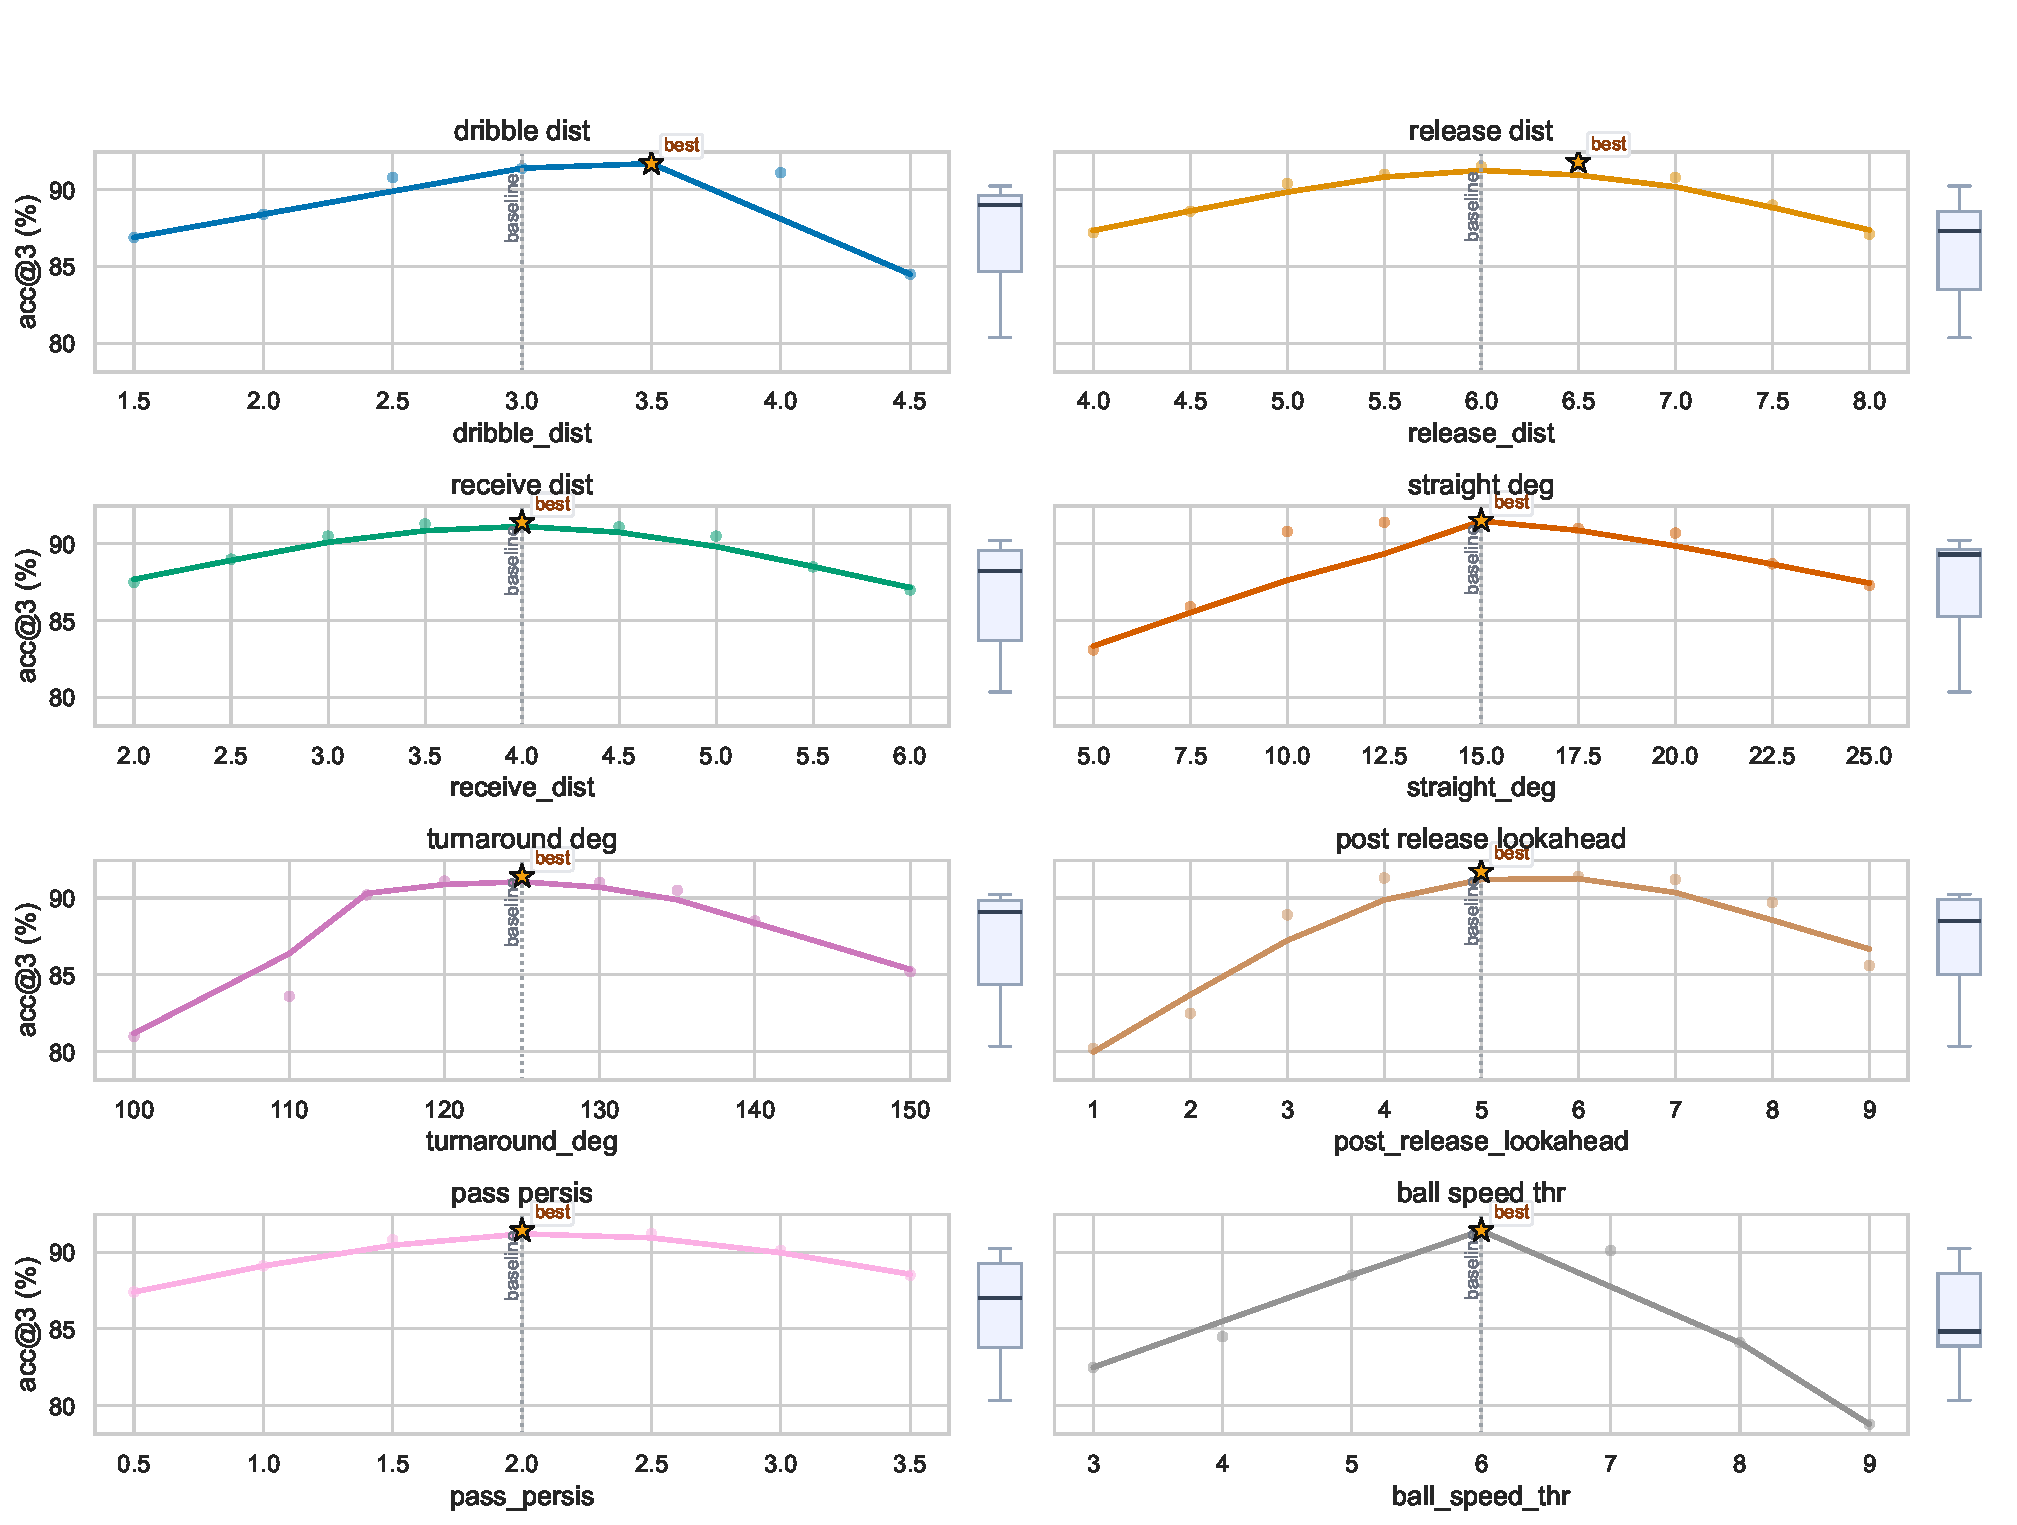
\includegraphics[width=\linewidth]{Fig/nba/llm_action_sensitivity_acc3_from_csv.pdf}
  \caption{NBA: sensitivity analysis of LLM-guided action parameters (Acc@3). The star marks the selected value; the vertical dashed line shows the LLM prior suggestion.}
  \label{fig:nba_action_sens}
\end{figure}

\subsection{Latent Mental State Cardinality}
\label{Sec:D2}

We further study the cardinality of the discrete mental state $m$ (semantic interpretations in Appendix~\ref{Sec:B5}). 
For \textbf{NBA}, \textbf{Car-Following}, and \textbf{Atari–Berzerk}, Figures~\ref{fig:z_effect_nba}–\ref{fig:z_effect_atari} plot three views: (left) Acc@5 versus epochs, (middle) training time, and (right) inference latency. 
Increasing the number of states improves early learning but may increase compute; a modest cardinality yields a favorable accuracy–efficiency tradeoff (the selected $m$ per dataset is reported in Appendix~\ref{Sec:B5}). 
For \textbf{DDXPlus}, the number of states is fixed per the experimental log, so no sweep is reported.

\begin{figure*}[t]
  \centering
  
\includegraphics[width=\linewidth]{Fig/nba/nba_z_effect.pdf}
  \caption{NBA: effect of the number of mental states $m$ on Acc@5, training time, and inference latency.}
  \label{fig:z_effect_nba}
\end{figure*}

\begin{figure*}[t]
  \centering
  
\includegraphics[width=\linewidth]{Fig/car_following/nba_z_effect.pdf}
  \caption{Car-Following: effect of the number of mental states $m$ on Acc@5, training time, and inference latency.}
  \label{fig:z_effect_car}
\end{figure*}

\begin{figure*}[t]
  \centering
  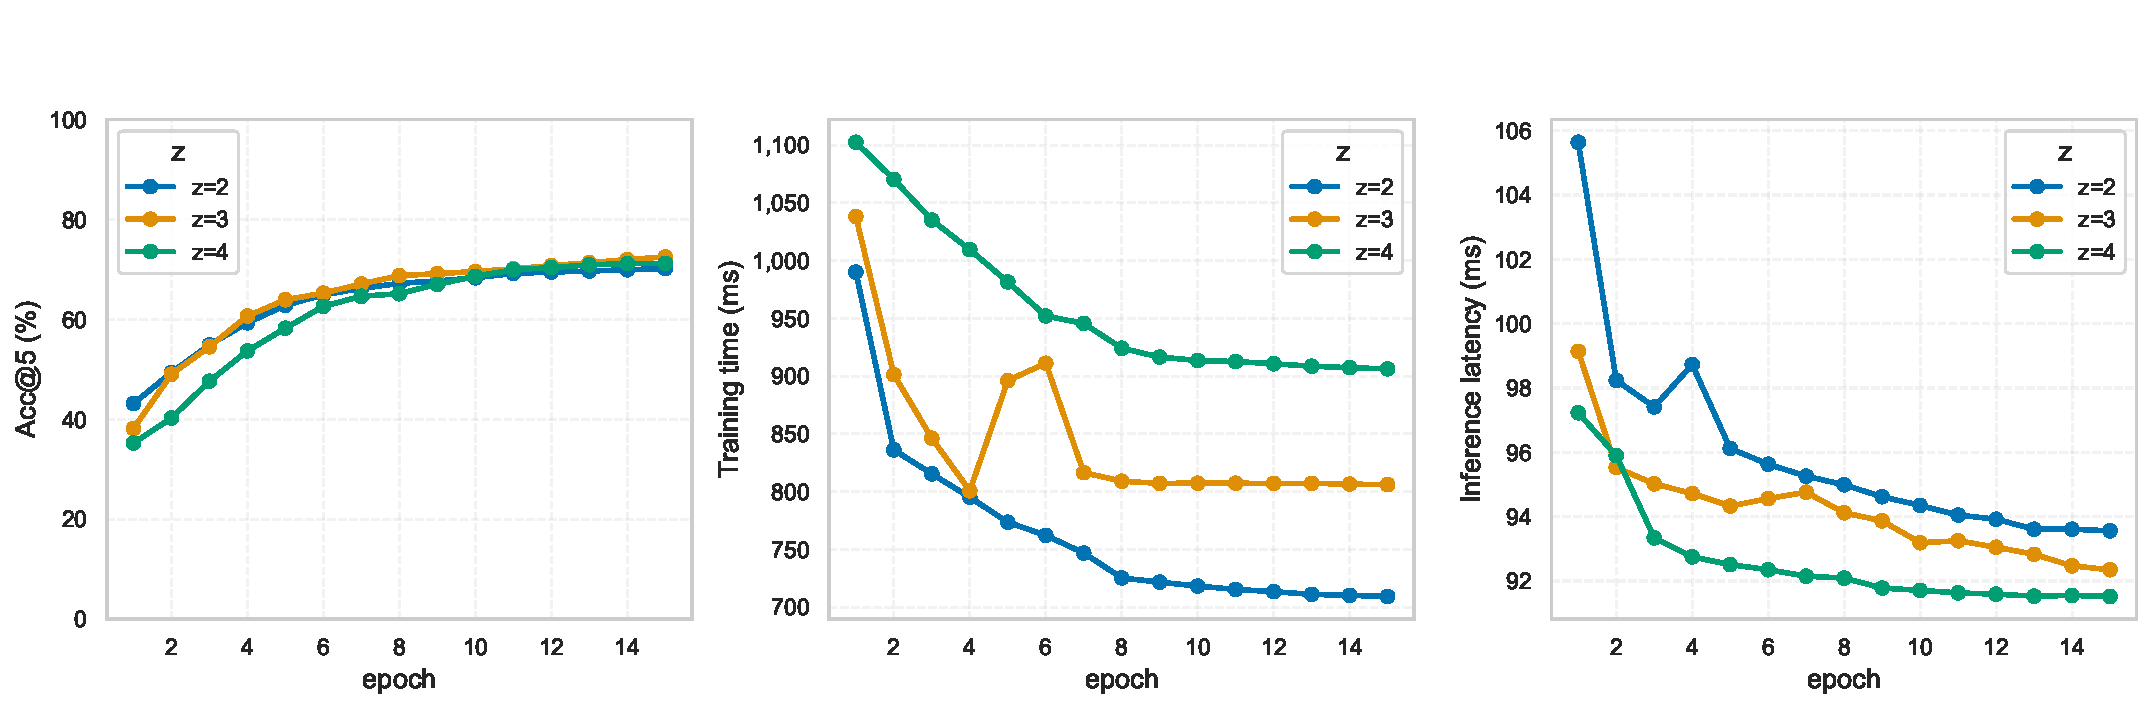
\includegraphics[width=\linewidth]{Fig/Atari/nba_z_effect.pdf}
  \caption{Atari–Berzerk: effect of the number of mental states $m$ on Acc@5, training time, and inference latency.}
  \label{fig:z_effect_atari}
\end{figure*}

\subsection{LLM Prompts}
\label{Sec:D3}

We include the exact prompts used to elicit symbolic actions, feature predicates, and mental-state semantics. 



%=================== NBA ===================%
\noindent\textbf{NBA (feature construction + action definition + $z$ design).}\\[-0.3em]
\begin{PromptBox}
You are given NBA play-by-play frames, where each frame contains only the 2D
coordinates of 11 entities (the ball + 10 players) with timestamps, plus team and
ball-possession labels. No actions or features are predefined; only raw positions
are available.

Your task is to:

1. Inspect the distribution of the data and decide how many latent z states
   should be used. For each z, provide a semantic interpretation (e.g.,
   habitual/exploit, explore, subgoal switch) and define triggering conditions.

2. Define a set of interpretable basketball actions (e.g., straight move, left turn,
   right turn, turnaround, dribble, shoot, pass) and specify the measurable
   thresholds (angles, distances, speeds, frame persistence, ball speed) for
   classifying them.

3. Construct interpretable features from raw coordinates, such as speed, heading
   angle, relative distances, angle changes, and possession switches, with formulas
   and units.

4. For each threshold, provide default values and ranges
   (conservative / standard / aggressive settings).
\end{PromptBox}

%=================== Car-Following ===================%
\noindent\textbf{Car-Following (feature construction + $z$ design).}\\[-0.3em]
\begin{PromptBox}
You are given car-following data represented as sequences of discrete regimes.
The regime set is fixed as {Fa, Fd, C, A, D, F, S}, where each regime represents
a specific driving behavior such as cruising, accelerating, or decelerating.
Only these sequences are available, with no additional environment variables.

Your task is to:

1. Inspect the distribution of these regime sequences and decide how many latent
   z states should be defined. Provide semantic interpretations for each z
   (e.g., conservative driving, aggressive driving, bursty switching).

2. Design interpretable features that can be derived from the regime sequences,
   such as switching rate, run length of consecutive regimes, time since last
   switch, or ratios of sudden accelerations/decelerations. Provide formulas for
   these features.

3. For each feature, propose thresholds with default values and ranges
   (conservative / standard / aggressive).
\end{PromptBox}

%=================== DDXPlus ===================%
\noindent\textbf{DDXPlus (feature construction suggestions; actions fixed; $z$ given = severity 1--5).}\\[-0.3em]
\begin{PromptBox}
You are given patient diagnostic trajectories from the DDXPlus dataset.
Each trajectory consists of sequential actions of two types:
ASK: querying a symptom, sign, or test and DIAG: issuing a diagnosis.
The latent z state (severity from 1 to 5) is already provided by the dataset,
and the action vocabulary is fixed.

Your task is to:

1. Suggest how to construct interpretable features from the raw evidences.
   For example, propose ways to group evidences into thematic clusters
   (such as URTI core symptoms, systemic symptoms, or risk factors)
   or embed them into low-dimensional representations.

2. Provide recommendations for feature engineering choices such as
   embedding dimension, normalization, or grouping heuristics.
\end{PromptBox}


%=================== Atari ===================%
\noindent\textbf{Atari–Berzerk ($z$ design from pixels; actions fixed).}\\[-0.3em]
\begin{PromptBox}
You are given raw Atari Berzerk gameplay frames, each being a 128×128
grayscale or RGB image. The action space is fixed at 18 discrete actions
(combinations of movement and firing). No explicit state features are provided;
the world model will learn directly from pixels.

Your task is to:

1. Based on typical human gameplay strategies, decide how many latent z states
   should be used.

2. Provide a semantic interpretation for each z (e.g., exploit = repetitive safe
   movement, explore = trying rare actions or new regions, danger = escaping when
   enemies cluster).

3. Estimate the relative prevalence of each z (e.g., most frames are exploit,
   fewer are explore or danger).
\end{PromptBox}


\section{Limitations and Broader Impact}
\label{sec:limitations}

While our framework demonstrates strong performance and interpretability across
diverse domains, several limitations remain. First, the rule extraction process
is still partly dependent on the quality of predicates or action abstractions
available in each dataset. Although our wake--sleep cycles mitigate this by
progressively refining rules, fully unsupervised discovery of symbolic structures
remains an open challenge. Second, our current design balances rules and active
inference at a single timescale; extending the framework to explicitly
multi-level hierarchies (e.g., subgoals and long-term planning) is a natural
next step. Third, although rule-based reasoning improves robustness on rare or
edge-case behaviors, its coverage is inherently sparse, and rule confidence
thresholds must be tuned to avoid spurious activations. Finally, our experiments
are conducted on curated benchmarks; evaluating the method in highly dynamic or
noisy real-world environments (e.g., human–robot collaboration, autonomous
driving in open traffic) remains important future work.

Despite these limitations, we believe the broader impact of our approach is
promising. By combining generative models with symbolic rules, the framework
offers a path toward \emph{transparent, human-interpretable decision-making},
potentially increasing trust in safety-critical applications such as healthcare,
transportation, and multi-agent coordination. The ability to capture both
frequent and rare behaviors in a complementary manner also suggests that our
method can generalize to domains where data imbalance or uncertainty is
prevalent. More broadly, the work illustrates how insights from cognitive
science---such as rule-guided inference and predictive coding---can inspire
practical algorithms that balance performance with interpretability. We hope
this line of research stimulates further integration of symbolic reasoning and
active inference in future intelligent systems.

\section{Use of LLMs}
\label{appendix_sec:use_of_llms}

In this paper, LLMs were used solely for writing polishing in several paragraphs, like the Experiment section. All the key ideas, proofs, research, and writing are created completely by human authors.

\iffalse
\section{Experiments}
\label{sec:experiments}

To comprehensively evaluate our model in distinct behavioral scenarios, we conducted large-scale experiments on on NBA SportVU dataset for player action modeling and Car-Following dataset for driver behavior modeling. Each experiment comprised a \emph{Blockwise Wake–Sleep} pre-training phase and a \emph{Full Wake–Sleep} training phase. In addition to the action-prediction accuracy and time efficiency, we recorded the number of rules, rule-trigger rate, rule-fusion probability, and free energy change to highlight the dynamic contributions of our architecture and its modules.

\subsection{Experimental Setup}

\paragraph{Dataset} We consider two real-world datasets: {\it i) NBA SportVU\footnote{https://github.com/linouk23/NBA-Player-Movements}}~\citep{kambhamettu2024quantifying}: It is collected by NBA using the SportVU tracking system, which reports the trajectories of the ten players and the ball in real basketball games. Each trajectory contains the
2D positions and velocities of the offensive team, consisting of five players. We follow similar data prepossessing strategy as \cite{cao2023discovering} and extract 20000 NBA player action sequences with action set containing [straight, left,
right, turn around, dribble, shoot, pass].
{\it ii) Car-Following\footnote{https://github.com/RomainLITUD/Car-Following-Dataset-HV-vs-AV}}~\citep{li2023large}: It is processed from Lyft level-5 open dataset~\citep{houston2021one}, a large-scale dataset of high-resolution sensor data collected by a fleet of $20$ self-driving cars, which includes $1000+$ hours of perception and motion data collected over a $4$-month period from urban and suburban environments along a fixed route in Palo Alto, California. We We extract 2000 car-following behavior sequences with action set containing [free acceleration, cruising, acceleration following, deceleration following, constant speed following]. 

\paragraph{Baselines} We choose state-of-the-art baselines considering three different fields: {\it i) Logic based Models}: RNNLogic~\citep{qu2020rnnlogic}, STLR~\citep{cao2023discovering}, and LaTee~\citep{song2024latent}. {\it ii) Deep Neural Models}: HYPRO~\citep{xue2022hypro}, XTFormer~\citep{xiao2025xtsformer}, and Re-Net~\citep{jin2019recurrent}, and {\it iii) Active Inference Models}: DAI~\citep{ccatal2020learning} and DAI-MC~\citep{fountas2020deep}.

\paragraph{Metrics} We adopt two metrics for evaluation: {\it i) Acc$@K$}:
It quantifies action prediction accuracy across varying time steps, demonstrating precision in both short-term (e.g., $K=1$) and long-term (e.g., $K=3\ \text{or} \ 5$) predictive scenarios. {\it ii) Time efficiency}: Our evaluation protocol comprises two experimental scenes. For baseline comparison, we use converged training time cost (denoted as {\it TC (h)}) to ensure fair performance assessment against baselines. For ablation study, we use component-level analysis employing time-per-step metrics (denoted as {\it TPS (s)}) to quantify the impact of separate modules within our model on overall training efficiency.

%%%%%%%%%% Move to appendix
% \paragraph{Parameter Settings} To ensure reproducibility and fair comparison, we adopted the following core configurations for both experiments (NBA SportVU and Car-Following); other specific parameters are detailed in Appendix~3.

% For NBA SportVU, we randomly sampled 20 events from 100 games, and for each event we traversed all 10 players, yielding 16\,000 training samples and 4\,000 test samples. We used a history length of $H=5\ (\approx2\mathrm{s})$ to predict a future length of $H=10\ (\approx4\mathrm{s})$. The world model is 42-dimensional, based on the directional kernel distances of the 10 teammates plus a shot-urgency clock. Predicates were constructed from single-frame 6-dimensional relational features: the distances from the three nearest defenders to the ball and the handler’s distance $d_{\mathrm{rim}}$ and angle $\theta$ to the rim. Since the straight‐line action predicate (“\(\mathrm{straight}\)”) is overly prevalent and would confound our ablation study, all predicate combinations triggering a straight action were ignored. 

% For Car-Following, we retained only events with action-sequence length \(\ge8\), yielding 19\,520 training samples and 2\,500 validation samples. Only discrete action sequences were used, with no additional environmental observations (hence no world model or corresponding VFE). Predicates were taken as historical action subsequences of length 3–4.

% As for training schedules of both datasets, pre-training used 10 blocks and 5 epochs; full training used 20 epochs. In all cases, batch size was 32, and learning rates were \(1\times10^{-4}\) (NBA) and \(1\times10^{-3}\) (Car-Following). 



\subsection{Experimental Results and Analysis}


\begin{figure*}[!t]
  \centering
  
\includegraphics[width=1.0\textwidth]{ICLR 2026/Fig/Training.pdf}
  \vspace{-20pt}
  \caption{Training results.}
  \label{fig:training}
\end{figure*}

\begin{figure*}[!t]
  \centering
  \includegraphics[width=1.0\textwidth]{ICLR 2026/Fig/Validation.pdf}
  \vspace{-15pt}
  \caption{Validation results and Top-5 rules in pretraining and full training process.}
  \label{fig:validation}
\end{figure*}


\paragraph{Results of NBA SportVU Dataset}
The model convergence and detailed results are shown in Fig.~\ref{fig:training} and Fig.~\ref{fig:validation}. In the pre-training phase, the rule count grew rapidly from 0 to 20–25, then converged at 24–29 after dynamic decay and pruning, ensuring a compact pool of high-confidence rules. The rule-trigger rate stabilized at 16–20\%, and the fusion probability (including rollout fusion) was slightly higher at 18–20\%. On the test set, as rule count and model parameters jointly optimized, both short-term and less long-term prediction accuracies improved significantly. All components of \(\Delta F\) (VFE, EFE, and KL) showed a downward trend, indicating that the model increasingly compressed its generative posterior fit to the observation sequences. During full training, repeated Wake–Sleep cycles yielded further fine-tuning: Acc$@K$ improved steadily, inference speed stabilized, trigger and fusion rates remained consistent, and total \(\Delta F\) along with its components continued decreasing, reflecting further refinement of the world model and belief distribution.

\paragraph{Results of Car-Following Dataset}
See Figures in Appendix for full results and convergence. Similarly, across both pre-training and full-training phases, rule count rose quickly and stabilized at 169–174. The rule-trigger rate stabilized at 65–70\%, and fusion probability reached 93–94\% (the excess over the trigger rate corresponds to multi-rule rollout fusion), demonstrating the substantial contribution of the rule mechanism on this dataset. On the validation set, both near-term and long-term prediction accuracies exhibited stable and reliable performance.

\begin{table}[ht]
\centering
\small
\label{tab:baseline}
\begin{tabular}{clcccccccc}
\toprule

\multirow{2}{*}{\textbf{Category}} & \multirow{2}{*}{\textbf{Method}} & \multicolumn{4}{c}{\textbf{NBA SportVU}} & \multicolumn{4}{c}{\textbf{Car-Following}} \\
% \hline

% & & \multicolumn{4}{c}{\textbf{NBA SportVU}} & \multicolumn{4}{c}{\textbf{Car-Following}} \\
\cmidrule(r){3-6}\cmidrule(l){7-10}
& & Acc@1 & Acc@3 & Acc@5 & TC (h) 
& Acc@1 & Acc@3 & Acc@5 & TC (h) \\
\midrule
\multirow{3}{*}{\shortstack{Logic\\Based}} & RNNLogic & 67.2\% & 60.5\% & 51.8\% & 2.2 & 72.3\% & 68.4\% & 57.5\% & 0.9 \\
& STLR & 75.2\% & 74.6\% & 70.2\% & 3.3 & 78.9\% & 76.5\% & 75.0\% & 1.2 \\
& LaTee & 78.5\% & 73.3\% & 64.5\%   & 4.6 & 82.3\% & 74.7\% & 71.8\%   & 2.4 \\
\hline
\multirow{3}{*}{\shortstack{DeepNN\\Based}} & HYPRO & 76.2\% & 75.3\% & 71.6\% & 2.8 & 77.3\% & 75.8\% & 72.6\% & 1.4 \\
& XTFormer & 64.6\% & 58.8\% & 42.3\% & 2.5 & 68.2\% & 53.5\% & 44.5\% & 1.6 \\
& Re-Net & 72.1\% & 68.4\% & 62.0\% & 2.3 & 76.3\% & 70.7\% & 67.2\% & 1.1 \\
\hline
\multirow{2}{*}{\shortstack{Active\\Inference}}& DAI & 75.3\% & 70.5\% & 62.3\% & 1.2 & 78.8\% & 73.3\% & 68.5\% & 0.6 \\
& DAI-MC & 82.3\% & 80.6\% & 76.4\% & 1.5 & 84.5\% & 82.8\% & 80.1\% & 0.7 \\
\hline
-- & \textbf{Ours} & 96.3\% & 94.6\% & 93.1\% & 2.2 & 98.9\% & 95.4\% & 93.8\% & 1.3 \\
\bottomrule
\end{tabular}
\caption{Comparison with standard baselines on NBA SportVU and Car-Following datasets in prediction tasks.}
\label{tab:prediction}
\end{table}

\paragraph{Analysis} We conducted an in-depth comparison between our model and relevant baselines (Table~\ref{tab:prediction}). Although our model’s convergence speed (measured by Acc$@1\ge85\%$ on the validation set) was slower than some lightweight methods, it delivered markedly superior accuracy for action-type prediction, especially over longer horizons. By leveraging Beam Search and merging single-rule hits, no-rule hits, and multi-rule hits in decision paths, our inference speed became more robust. To further illustrate the interpretability and practical benefits of our decision model, we present the actual inference trajectories on real data in Figures of Appendix. From these experiments, we highlight the following strengths: {\it i)} \textbf{Synergistic gains of alternating Wake–Sleep}: in the Wake phase, rule matching and multi-step rollout generate candidate rules; in the Sleep phase, world model parameters and the policy network are optimized. Alternating these phases ensures convergence of ``low-level parameter learning'' while continuously discovering and refining ``high-level symbolic rules,'' forming a positive feedback loop. {\it ii)} \textbf{Insights from free energy decomposition}: All three components—VFE, EFE, and KL divergence—decreased significantly during training, confirming that the model compresses its internal representation while maintaining predictive accuracy.
{\it iii)} \textbf{Efficiency and interpretability of the rule module}: During pre-training, a set of high-confidence rules is quickly accumulated, covering many decision needs online and dramatically reducing multi-step search calls. Rule visualizations (Fig.~\ref{fig:training}) both reflect domain knowledge and afford high interpretability.

These results demonstrate that biologically inspired Wake–Sleep, rule-guided active inference effectively integrates statistical learning with symbolic induction in complex dynamic scenarios. Our multi-decision switching mechanism (single-rule direct trigger, multi-rule fusion, no-rule rollout) balances efficiency and flexibility. Across accuracy, free energy convergence, online inference latency, and interpretability, our framework outperforms or matches state-of-the-art methods, validating its advantages for modeling human behavior. 


\begin{wrapfigure}{r}{0.6\textwidth}
    \centering

\includegraphics[width=0.60\textwidth]{ICLR 2026/Fig/ablation.pdf}
    \vspace{-20pt}
\caption{Ablation Study.}
\label{fig:ablation_study}
\end{wrapfigure}

\subsection{Ablation Study}
\vspace{-5pt}
We conducted an ablation study to assess the importance of different components, ablating the following modules: {\it i) Habitual Engine (rule matching)}, {\it ii) Free Energy}, {\it iii) Active Inference}, and {\it iv) Switching Sampling Mechanism} for both both NBA SportVU and Car-Following. The results are presented in Fig.~\ref{fig:ablation_study}), from which one can observe that {\it Habitual Engine} carries high-confidence rules distilled in the Wake phase, instantly triggering correct actions in familiar scenarios. It greatly shortens query time and boosts short-term accuracy. Removing it causes a dramatic accuracy drop on Car-Following, underscoring its importance for real-time control. Removel of {\it Free Energy} cause the lose regularization of the belief distribution and environment reconstruction constraint, disabling the rule engine and unbalancing the model between policy and world model—leading to declines in both performance and efficiency. For {\it Active Inference}, by evaluating global \(\Delta F\), it drives the rollout/search process, balancing long-term planning and short-term exploration. Without it, decisions devolve into greedy site-based choices, losing long-range consistency. For {\it Switching mechanism}, differentiates exploratory and exploitative actions to produce more realistic decision-making and enhances interpretability. Although removing it slightly increases short-term accuracy in NBA, it degrades overall performance in the more complex Car-Following environment, indicating its critical role in adaptive decision selection.

Thus, these modules jointly form the model, improving accuracy and inference efficiency. In dynamic scenarios, the framework effectively integrates symbolic rules and deep models, balancing real-time responsiveness with long-term planning, and offering significant engineering and cognitive-science value.


\section{Conclusion}
\label{sec:conclusion}
\vspace{-5pt}
we propose a novel cognitive framework in which agents iteratively update their internal world models based on historical data through optimization, and use these models to plan and select future actions. The experimental results demonstrate that our model can capture key aspects of human behavior as well as enhance interpretability.
\fi



%%%%%%%%%%%%%%%%%%%%%%%%%%%%%%%%%%%%%%%%%%%%%%%%%%%%%%%%%%%%
\iffalse
\newpage
\appendix

\section*{Appendix Overview}
\begin{itemize}
  \item Section~\ref{Sec:A} presents the overall Wake–Sleep algorithm, including pseudocode for state reconstruction, belief updating, candidate rule extraction, model parameter optimization, etc. (Algorithms~\ref{alg:rule-guided-active-inference}).
  \item Section~\ref{Sec:B} describes the Beam Search planning method (Algorithm~\ref{alg:beam-search}) and the policy model (online reasoning, Algorithm~\ref{alg:online-reasoning}), detailing how exploration–exploitation switching and rule‐guided decisions are integrated.
  \item Section~\ref{Sec:C} provides supplementary experimental results: key hyperparameter settings (Table~\ref{tab:exp-params}), action classification and predicate extraction procedures for both Car‐Following and NBA SportVU domains, and additional training and validation curves on the Car‐Following dataset (Figures~\ref{fig:training}-~\ref{fig:validation}) with related analysis.
  \item Section~\ref{Sec:D} visualizes real‐world inference trajectories on NBA SportVU (Figure~\ref{fig:nba_timeline}) and Car‐Following (Figure~\ref{fig:car_timeline}) datasets, illustrating rule‐match outcomes, intention segmentation, backtracking events, and predicted actions in both map and time‐series views.
  \item Section~\ref{Sec:E} elaborates the internal mechanics of the Wake and Sleep phases (Algorithm~\ref{alg:wake-phase}-~\ref{alg:sleep-phase}), covering candidate‐rule pool construction, predicate generation, rule abstraction, confidence updating, and the joint free‐energy minimization objective.
  \item Section~\ref{Sec:F} outlines our two‐stage training schedule: blockwise pretraining (Algorithm~\ref{alg:blockwise-training}) for rapid initialization across data blocks, followed by full Wake–Sleep training (Algorithm~\ref{alg:full-training}) on the entire dataset for iterative refinement.
  \item Section~\ref{Sec:G} discusses the limitations of our framework, including domain specificity of mined rules, sensitivity to hyperparameters, computational overhead, reliance on world‐model accuracy, and the absence of formal convergence guarantees.
  \item Section~\ref{Sec:H} examines broader impact considerations, highlighting interpretability and safety benefits, risks of biased rule mining, privacy implications of trajectory data, and the environmental footprint of Wake–Sleep cycles and multi‐step planning.
\end{itemize}


\section{Wake-sleep Algorithm}
\label{Sec:A}
The agent alternates between a \emph{Wake Phase}, in which active inference is employed to perform state reconstruction, belief updating, and candidate rule extraction, and a \emph{Sleep Phase}, where model parameters are optimized by minimizing joint free energy and rule confidences are updated. Algorithm~\ref{alg:rule-guided-active-inference} summarizes this two-phase learning loop.

\begin{algorithm}[htbp]
\caption{Rule‐Guided Active Inference via Wake–Sleep}
\label{alg:rule-guided-active-inference}
\begin{algorithmic}[1]
\Require Trajectories $\mathcal{D}$, window length $H$, rollout depth $P$, thresholds $\delta_F$, $\delta_O$
\Ensure Learned parameters $(\phi_{\rm env},\phi_{st},\theta_{\rm inf},\theta_{\pi})$ and rule set $R$
\State Initialize $\phi_{\rm env},\phi_{st},\theta_{\rm inf},\theta_{\pi}$ randomly; $R\leftarrow\emptyset$
\For{each Wake–Sleep cycle}
\State \textbf{Wake Phase:} (more details in Appendix~\ref{sec:Wake})
  \For{each trajectory $\tau\in\mathcal{D}$ and timestep $t=H,\dots,|\tau|$}
    \State (1) Predict next observation: $\hat O_t=f_{\rm env}(O_{t-H+1:t-1},a_{t-H+1:t-1};\phi_{\rm env})$
    \State (2) Reconstruct state: $S_t=f_{st}(O_{t-H+1:t-1},\hat O_t,a_{t-H+1:t-1},\theta_{t-H+1:t-1};\phi_{st})$
    \State (3) Update belief: sample $\theta_t\sim q(\theta_t\mid S_t,\theta_{t-1},O_t;\theta_{\rm inf})$
    \For{each candidate path $\mathbf{a}_{t:t+P-1}$}
      \State (4.1) Compute cumulative free energy:
      $$F_{\rm path}=\sum_{k=0}^{P-1}F_{t+k} $$
      \State (4.2) Compute improvement:  $\Delta F = F_{\rm baseline}-F_{\rm path}$  
      
  \Comment{$F_{\rm baseline}$ is the cumulative free energy of the reference (e.g.\ MAP) of length \(P\).}
    \EndFor
    \State (5) Harvest high-value rules:
    $$R\leftarrow R \;\cup\;\{(C_i\to a_i)\mid \Delta F\ge\delta_F,\;\mathrm{std}(O)\ge\delta_O\}$$
  \EndFor
\State \textbf{Sleep Phase:} (more details in Appendix~\ref{sec:Sleep})
  \State (1) Generate synthetic trajectories via current world model
  \State (2) Minimize joint free energy:
  \[    F=\alpha\,\mathrm{VFE}_t+\beta\,\mathrm{EFE}_t+\gamma_{t}\,D_{\mathrm{KL}}\bigl[q(\theta_{t-1})\|q(\theta_t)\bigr]
  \]
  \State (3) Model optimization: Update $(\phi_{\rm env},\phi_{st},\theta_{\rm inf},\theta_{\pi})$ by gradient descent
  \State (4) Update rule confidences: $conf_i\leftarrow(1-\eta)conf_i+\eta\Delta F_i$
  \State (5) Prune low-confidence rules
\EndFor
\end{algorithmic}
\end{algorithm}
\noindent\textbf{Note 1}: All thresholds ($\delta_F,\delta_O$), decay factor $\eta$, weights $\alpha,\beta,\gamma$, rollout depth $P$, and other hyperparameters are detailed in Appendix~\ref{Sec:Parameter}.

\noindent\textbf{Note 2}: The Wake–Sleep two-phase cycle establishes a positive feedback loop between low-level parameter learning and high-level symbolic rule discovery, balancing flexible planning with efficient habitual decision-making. The models and rules obtained from each cycle (See Appendix~\ref{Sec:D} for examples) are used with the Beam Search algorithm (Appendix~\ref{Sec:Beam search}) to implement high-efficiency, high-accuracy Online Reasoning (Appendix~\ref{Sec:Reasoning}).


\section{Beam Search Method}
\label{Sec:B}
In our high-level active inference framework (Appendix~\ref{Sec:Reasoning}), we introduce the beam search method to let the agent quickly explore a few of the most promising multi‐step action sequences without evaluating every possibility, so it can plan flexibly under uncertainty and symbolic rule constraints in real time. Especially in scenarios where no single habit rule applies, the agent must plan over multiple steps to minimize expected free energy. The Beam Search subroutine (Appendix~\ref{Sec:Beam search}) is conditioned on the exploration–exploitation switch $z_t$ computed in the reasoning policy: when $z_t=1$ (explore), candidate expansions within the beam are sampled probabilistically to encourage diversity; when $z_t=0$ (exploit), expansions favor top-scoring actions to focus on high-utility trajectories.


\subsection{Beam Search Algorithm}
\label{Sec:Beam search}
The Beam Search procedure (Algorithm~\ref{alg:beam-search}) maintains a fixed-width beam of partial action sequences, expands each by appending new actions according to rule matches or "uncertainty-utility"-based sampling, and prunes to the top-$B$ sequences by cumulative score. This balances exploitation of high-value trajectories with exploration under uncertainty.

\begin{algorithm}[htbp]
\caption{Beam Search for Action Sequence Forward Planning}
\label{alg:beam-search}
\begin{algorithmic}[1]
\Require Rule set $R$, utility function $U(\theta,S,a)$, initial state $(S_t,\theta_t)$, beam width $B$, rollout depth $D$, switch threshold $\tau$, weights $w_\theta,w_s$, state summary $H(S)$, free‐energy weight $\lambda$
\Ensure Next action $a_t$ when no rule matched
\State Initialize beam:
  $\mathcal{B}^0 \gets \{(\emptyset,\,0,\,S_t,\,\theta_t)\}$
\For{$d=1,\dots,D$}
  \State $\mathcal{B}^d \gets \emptyset$
  \For{each $(\mathbf{a},s,S_{d-1},\theta_{d-1})\in\mathcal{B}^{d-1}$}
    \State // 1. Compute switch (Eq.~10)
    \State $p_{\rm explore}\gets \sigma\bigl(w_\theta^\top\theta_{d-1}+w_s^\top H(S_{d-1})\bigr)$
    \State $z\gets\mathbf{1}\{p_{\rm explore}>\tau\}$
    \If{rule $(C\to a_r)\in R$ matches history}
      \State $a'\gets a_r$, \ $p_a\gets1$
    \Else
      \If{$z=1$}  \Comment{exploration (Eq.~11)}
        \State sample $a'\sim p(a\mid\theta_{d-1},S_{d-1},z=1)$,\quad
              $p_a\gets p(a'\mid\theta_{d-1},S_{d-1},z=1)$
      \Else      \Comment{exploitation (Eq.~12)}
        \State sample $a'\sim p(a\mid\theta_{d-1},S_{d-1},z=0)$,\quad
              $p_a\gets p(a'\mid\theta_{d-1},S_{d-1},z=0)$
      \EndIf
    \EndIf

    \State // 2. Roll out one step
    \State $(S_d,\theta_d)\gets\mathrm{Step}(S_{d-1},\theta_{d-1},a')$

    \State // 3. Compute free‐energy change
    \State $\displaystyle\Delta F \;=\; F(S_{d-1},\theta_{d-1}) \;-\; F(S_d,\theta_d)$

    \State // 4. Compute incremental score
    \If{$z=1$}
      \State $\displaystyle\Delta s \;=\; \log p_a 
        \;+\;\bigl(w_\theta^\top\theta_{d-1}+w_s^\top H(S_{d-1})\bigr)
        \;+\;\lambda\,\Delta F$
    \Else
      \State $\displaystyle\Delta s \;=\; \log p_a 
        \;+\; U(\theta_{d-1},S_{d-1},a')
        \;+\;\lambda\,\Delta F$
    \EndIf

    \State Add $(\mathbf{a}\cup\{a'\},\,s+\Delta s,\,S_d,\,\theta_d)$ to $\mathcal{B}^d$
  \EndFor
  \State Prune beam: keep top-$B$ entries of $\mathcal{B}^d$ by score
\EndFor
\State Select best 
  $(\mathbf{a}^*,s^*) 
     = \mathop{\arg\max}{(\mathbf{a},s,\ldots)\in\mathcal B^D}$.
\State \Return first action $a_t=\mathbf{a}^*_1$
\end{algorithmic}
\end{algorithm}


\noindent\textbf{Note}:  
- This Beam Search is invoked only when no habitual rule applies (see Algorithm~\ref{alg:online-reasoning}). 

- At each look‐ahead step it recomputes  
  \(\displaystyle p_{\rm explore}=\sigma\bigl(w_\theta^\top\theta + w_s^\top H(S)\bigr),\quad 
     z=\mathbf1\{p_{\rm explore}>\tau\}.\)  

- If a rule applies, its action $a_r$ is taken with free‐energy bias \(\Delta F_{C\to a_r}\). Otherwise, exactly one action $a'$ is sampled only from the exploration pool (if \(z=1\), Eq.~11) or the exploitation pool (if \(z=0\), Eq.~12), and its probability \(p_a\) recorded.  
- Each candidate is rolled out: \((S_d,\theta_d)=\mathrm{Step}(\cdot)\), then scored via  
  \(\Delta s = \log p_a + U(\theta,S,a') + \lambda\,\Delta F.\)
  
- Here, \(U(\theta,S,a)\) is a problem‐specific utility measuring action value. For example, in NBA SportVU one can set  
  \[
    U(\theta_t,S_t,a_t) = w_1 S_t + w_2 \Delta S_t - w_3 \theta_t - w_4 cost(a_t),
  \]
  and use \(\sigma(U(\theta_t,s_t,a_t))\) as the action score.
  
- Hyperparameters \((B,D,\tau,w_\theta,w_s,\lambda)\) are detailed in Appendix~\ref{Sec:Parameter}.


\subsection{Online Reasoning}
\label{Sec:Reasoning}
The overall online decision‐making policy combines instantaneous rule‐based decisions with far‐sighted planning (active inference) when necessary. Algorithm~\ref{alg:online-reasoning} details the three decision pathways:

\begin{enumerate}[label=(\arabic*)]
  \item \textbf{Single‐rule hit:} apply the unique matched habitual rule immediately.
  \item \textbf{Multi‐rule hit:} compute adjusted free energies for all matched rules, then plan over the corresponding rule actions via multi‐step Beam Search.
  \item \textbf{No‐rule hit:} if no rule applies, invoke the full Beam Search planner (Algorithm~\ref{alg:beam-search}) over the entire action set.
\end{enumerate}

\begin{algorithm}[htbp]
\caption{Active Inference–based Online Reasoning via Rule‐Guided Policy}
\label{alg:online-reasoning}
\begin{algorithmic}[1]
\Require Observations $O_{t-H+1:t-1}$, past actions $a_{t-H+1:t-1}$, world model $f_{\rm env},f_{st}$, inference engine $q(\cdot;\theta_{\rm inf})$, rule set $R$, full action space $A$, Beam Search Planner
\Ensure Action $a_t$, policy parameters $\theta_{\pi}$
%
\State // 1. State reconstruction and belief update  
\State $\hat O_t = f_{\rm env}(O_{t-H+1:t-1},\,a_{t-H+1:t-1})$  
\State $S_t = f_{st}(O_{t-H+1:t-1},\,\hat O_t,\,a_{t-H+1:t-1})$  
\State $\theta_t \sim q(\theta_t \mid S_t,\,\theta_{t-1},\,O_t; \theta_{\rm inf})$
%
\State // 2. Habitual‐rule lookup  
\State $R_t = \{\,r\in R : \mathrm{antecedent}(r)\text{ matches }O_{t-H+1:t}\}$
\If{$|R_t|=1$} \Comment{single‐rule hit}
  \State $a_t = \mathrm{action}(\mathrm{unique}(R_t))$
  \State \Return $a_t$
\ElsIf{$|R_t|>1$} \Comment{multi‐rule hit}
  \State // 2.1 Compute adjusted free energy for each rule  
  \For{each $r\in R_t$}
    \State $F_t(r)=\alpha\,\mathrm{VFE}(r)+\beta\,\mathrm{EFE}(r)+\gamma_t\,D_{\mathrm{KL}}$  
    \State $\tilde F_t(r)=F_t(r)-\lambda\ln w_r$
  \EndFor
  \State // 2.2 Restrict planning to matched‐rule actions  
  \State $A_r=\{\mathrm{action}(r)\mid r\in R_t\}$
  \State // 2.3 Multi‐step planning over $A_r$  
  \State $a_t = \mathrm{BeamSearch}(U,\,A_r,\,S_t,\,\theta_t,\,P,\,B,\,\tau)$
  \State \Return $a_t$
\Else \Comment{no‐rule hit}
  \State // 3. Full multi‐step Beam Search over all actions  
  \State $a_t = \mathrm{BeamSearch}(U,\,A,\,S_t,\,\theta_t,\,P,\,B,\,\tau)$
  \State \Return $a_t$
\EndIf
\end{algorithmic}
\end{algorithm}

\noindent\textbf{Note}:  
- This policy (Alg.~\ref{alg:online-reasoning}) implements §4.2.3 as follows:  
(1) a single‐rule hit triggers immediate habitual action;  
(2) a multi‐rule hit first biases each rule by its adjusted free energy $\tilde F_t(r)$, then invokes BeamSearch constrained to those rule actions;  
(3) a no‐rule hit invokes full BeamSearch for multi‐step, free‐energy‐based planning. Hyperparameters $P,B,\tau,\alpha,\beta,\gamma_t,\lambda$ are detailed in Appendix~\ref{Sec:Parameter}. 

- Moreover, in accordance with the active inference framework, at each decision point we execute only the first action of the planned sequence. This receding‐horizon control strategy enables continuous belief updating and adaptive replanning as new observations arrive, while still leveraging multi‐step free‐energy minimization.  


\section{Other Experiment Results}
\label{Sec:C}
\subsection{Specific Experimental Parameter Settings}
\label{Sec:Parameter}

Table~\ref{tab:exp-params} summarizes the main hyperparameters and settings used in our Car‐Following and NBA SportVU experiments.

\begin{table}[htbp]
\centering
\small
\setlength{\tabcolsep}{3pt} 
\caption{Key Hyperparameters and Settings}
\label{tab:exp-params}
\begin{tabularx}{\linewidth}{@{} l X X @{}}
\toprule
\textbf{Category} & \textbf{Car‐Following} & \textbf{NBA SportVU} \\
\midrule
\multicolumn{3}{@{}l}{\textbf{Dataset \& Actions}} \\
\quad \# train/val/test 
  & 19\,520/2\,500/– 
  & 16\,000/–/4\,000 \\
\quad Action classes
  & \makecell[tl]{7 (\{F,A,D,C,Fa,Fd,S\})}
  & \makecell[tl]{7 (\{straight, left, right,\\ turn\_around, dribble,\\ shoot, pass\})} \\
\midrule
\multicolumn{3}{@{}l}{\textbf{Model Architecture}} \\
\quad World \& state model
  & – 
  & \makecell[tl]{$f_{\rm env},f_{st}$ on 10 players\\+ clock} \\
\quad Belief inference
  & \makecell[tl]{Gaussian BiGRU\\(dim 16, hidden 14)}
  & \makecell[tl]{Gaussian Transformer\\(dim 32, hidden 116,\\ dropout 0.1)} \\
\midrule
\multicolumn{3}{@{}l}{\textbf{Free‐Energy Parameters}} \\
\quad Weights
  & \makecell[tl]{$\beta_z=1.0,\;\beta_a=1.0,$\\$\gamma_{kl}=0.1$}
  & \makecell[tl]{$\alpha=0.01,\;\beta=1.0,$\\$\gamma=0.5$} \\
\midrule
\multicolumn{3}{@{}l}{\textbf{Training Schedule}} \\
\quad Pre‐training
  & 10 blocks × 5 epochs/block
  & 10 blocks × 5 epochs/block \\
\quad Full training
  & \makecell[tl]{20 epochs, batch 32,\\lr $1\times10^{-3}$}
  & \makecell[tl]{20 epochs, batch 32,\\lr $1\times10^{-4}$} \\
\midrule
\multicolumn{3}{@{}l}{\textbf{Beam Search Planner}} \\
\quad Beam width $B$, rollout depth $P$
  & 5, 3
  & 5, 3 \\
\midrule
\multicolumn{3}{@{}l}{\textbf{Pruning Thresholds}} \\
\quad Free‐energy improvement
  & $\ge25\%$ 
  & $\ge25\%$ \\
\quad Free‐energy std (if used)
  & $\ge25\%$
  & - \\
\quad Confidence threshold
  & $\ge75\%$
  & $\ge75\%$ \\
\quad Minimum triggers
  & 2/100
  & 2/100 \\
\midrule
\multicolumn{3}{@{}l}{\textbf{Rule Parameters}} \\
\quad Rule length
  & 3–4
  & 1 \\
\quad Decay factor
  & 0.9
  & 0.9 \\
\quad Enhancement factor
  & $1+0.3$
  & $1+0.3$ \\
\bottomrule
\end{tabularx}
\end{table}

\bigskip
\noindent\textbf{Additional details:}
\begin{itemize}
  \item \textbf{Loss function:} Training is driven by the free‐energy objective (Eq.~9); an auxiliary cross‐entropy on action prediction can be added in our experiments but had negligible effect (it can be verified from the convergence graph).
  \item \textbf{Car‐Following specifics:} Since no world date is recorded, the observation‐reconstruction term since $f_{\rm env}$ is absent. Moreover, here we choose the past action sequence as our antecedent. Trough our test, rules of length 3–4 yielded best accuracy; shorter rules degraded performance.
  \item \textbf{NBA SportVU specifics:} Since the action "straight" occupies the nearly most of the action space, we exclude the “straight” action when mining rules to mitigate label imbalance especially for ablation study. Predicates include distances/angles of the three closest defenders and the ball‐handler’s distance/angle to the rim (details see Appendix~\ref{sec:action classification}).
\end{itemize}

\subsection{Action Classification and Predicate Extraction}
\label{sec:action classification}
\paragraph{Car‐Following.}  
In the Car‐Following experiments, we use the seven discrete acceleration labels provided by the original dataset, focusing on action order:  
\[
\{\mathrm{F},\mathrm{A},\mathrm{D},\mathrm{C},\mathrm{Fa},\mathrm{Fd},\mathrm{S}\},
\]  
standing for “following,” “acceleration,” “deceleration,” “cruising,” “free acceleration,” “free deceleration,” and “constant speed following,” respectively.  Since no world‐model observation function \(f_{\rm env}\) is available, we treat each candidate rule’s antecedent as the raw sequence of the previous 3–4 driver actions.  In other words, a rule is simply a predicate on the last \(k\in\{3,4\}\) action labels, e.g.\ \(\mathrm{if}\;\{A,D,C\}\to\mathrm{D}\).

\paragraph{NBA SportVU.}  
We define seven discrete basketball actions via analytic rules. Let $p_t\in\mathbb R^2$ be the player’s position, $b_t\in\mathbb R^2$ the ball position, and $h_t\in\mathbb R^2$ the unit‐heading vector (computed by normalizing $p_t-p_{t-1}$). Define constants
\[
D_{\rm dribble}=2\text{ ft},\quad
D_{\rm release}=6\text{ ft},\quad
D_{\rm receive}=2\text{ ft}.
\]
Then
\[
a_t = 
\begin{cases}
4,& \|p_t - b_t\|\le D_{\rm dribble},\\
6,& \|p_{t-1}-b_{t-1}\|\le D_{\rm dribble},\ \|p_t - b_t\|\ge D_{\rm release},
      \ \min_{j\neq\text{handler}}\|y^j_t-b_t\|\le D_{\rm receive},\\
5,& \|p_{t-1}-b_{t-1}\|\le D_{\rm dribble},\ \|p_t - b_t\|\ge D_{\rm release},
      \ \min_{j\neq\text{handler}}\|y^j_t-b_t\|>D_{\rm receive},\\
0,& \angle(h_{t-1},h_t)<\epsilon,\\
3,& \angle(h_{t-1},h_t)>\pi-\epsilon,\\
1,& \text{otherwise if }(h_{t-1}\times h_t)>0,\\
2,& \text{otherwise if }(h_{t-1}\times h_t)<0,
\end{cases}
\]
where $\epsilon=\pi/18$ (10°), and $y^j_t$ are defender positions.

To extract symbolic predicates, we compute for each historical frame $t=1,\dots,H$:

1. Soft direction–kernel features: for each opponent $j$ and basis direction
   $b_i\in\{(1,0),(0,1),(-1,0),(0,-1)\}$, we define
\[
\phi_{i,j,t}^{\mathrm{dir}}
= \exp\!\Bigl(-\tfrac{\|p_t - y^j_t\|^2}{2\sigma^2}\Bigr)
\,\max\bigl(b_i\!\cdot u^j_t,\,0\bigr),
\]
where 
\[
u^j_t = \frac{y^j_t - p_t}{\|y^j_t - p_t\|},
\quad
\sigma = 10.
\]

2. Relational distance/angle features: let $d_j = \|p_t - y^j_t\|$ and sort $d_{(1)} \le d_{(2)} \le d_{(3)}$; define
\[
\begin{aligned}
d_{\mathrm{rim}}
= \|p_t - r\|,  
\theta_{\mathrm{rim}}
= \operatorname{atan2}\bigl(r_{y} - p_{t,y},\,r_{x} - p_{t,x}\bigr),
d_{\mathrm{mean}}
= \frac{1}{\lvert\mathcal O\rvert - 1}
   \sum_{j\in \mathcal O \setminus \{\mathrm{handler}\}} d_j.
\end{aligned}
\]
Then form
\[
\phi_t^{\mathrm{rel}}
= \bigl[d_{(1)},\,d_{(2)},\,d_{(3)},\,d_{\mathrm{rim}},\,\theta_{\mathrm{rim}},\,d_{\mathrm{mean}}\bigr].
\]

We concatenate $\{\phi_{i,j,t}^{\mathrm{dir}}\}_{i,j}$ and $\phi_t^{\mathrm{rel}}$ to obtain a continuous feature vector $\phi_t$. Finally, each dimension of $\phi_t$ is discretized via precomputed bin edges as
\[
\mathrm{bin}_i
= \min\!\bigl(\,\max\!\bigl(\mathrm{digitize}(\phi_{t,i},\,\mathrm{edges}_i)\!-\!1,\,0\bigr),\;\lvert\mathrm{edges}_i\rvert - 2\bigr),
\]
yielding a tuple of integer predicates for rule mining and online reasoning.


\subsection{Results on the Car-Following Dataset}

\begin{figure*}[!t]
  \centering
  
\includegraphics[width=1.0\textwidth]{ICLR 2026/Fig/car_tra.pdf}
  \vspace{-20pt}
  \caption{Training curves on the Car-Following dataset.  \textbf{(Top)} Block-wise pretraining: cross‐entropy loss and total free‐energy converge rapidly, rule pruning count stabilizes around 170 with trigger‐rate $\approx 32\%$.  \textbf{(Bottom)} Epoch-wise fine‐tuning: further reduction in CE and FE, rule count holds at $\approx172$ with trigger‐rate $\approx33\%$.  \textbf{(Right)} Free‐energy decomposition across blocks: expected‐FE (EFE) and KL‐term both decrease, showing improved model fit and exploration–exploitation balance.}
  \label{fig:training}
\end{figure*}

\begin{figure*}[!t]
  \centering
  
\includegraphics[width=1.0\textwidth]{ICLR  2026/Fig/car_val.pdf}
  \vspace{-15pt}
  \caption{Validation performance on the Car-Following dataset \textbf{(Left)} vs.\ pretraining blocks: trigger rate rises from 62\% to $\approx70\%$, fusion‐probability remains $>85\%$, and Acc@1/3/5 climb to 98.9\%/95.4\%/93.8\% (TPS $\approx0.0101$s).  \textbf{(Middle)} vs.\ fine‐tuning epochs: trigger rate $\approx69\%$, fusion‐prob $>92\%$, Acc@1/3/5 reach 99.2\%/96.1\%/94.1\% (TPS $\approx0.0103$s).  \textbf{(Right)} Top‐5 learned rules in (blockwise) pretraining and full (epoch) training, showing high‐confidence, high‐weight habitual policies.}
  \label{fig:validation}
\end{figure*}

Figures~\ref{fig:training}–\ref{fig:validation} demonstrate that our Wake–Sleep framework rapidly discovers a compact, high‐quality rule set and jointly trains the world model and policy:
\begin{itemize}
  \item \textbf{Efficiency \& Accuracy.}  Acc@1 reaches $\mathbf{98.9\%}$ after 10 blocks and further to $\mathbf{99.2\%}$ after 10 epochs.  Acc@3/5 similarly exceed $94\%/90\%$ while average time per step~(TPS) remains low ($\approx$0.010\,s).
  \item \textbf{Rule Triggering.}  The trigger rate—the fraction of time steps covered by at least one rule—rises from 62\% to $\approx$70\% in pretraining and holds at $\approx$69\% in full training, yielding a Fusion‐Prob $>92\%$ of decisions guided by rules.
  \item \textbf{Interpretability.}  The top rules (Figure~\ref{fig:validation}) correspond to intuitive car‐following behaviors (e.g.\ “if bin pattern \{0,1,0\} then accelerate”), with high confidence and normalized weights, illustrating clear symbolic policies learned in tandem with the world model.
\end{itemize}

On the Car-Following benchmark, our method simultaneously achieves state‐of‐the‐art prediction accuracy, low inference latency, and yields an interpretable habitual rule set—validating the efficacy of the rule‐guided Wake–Sleep Active Inference approach in real‐world continuous control scenarios.




\section{Actual Inference Trajectories on Real Data}
\label{Sec:D}
\subsection{NBA SportVU Trajectories Display}
\label{sec:nba_display}

In this subsection, we illustrate a representative offensive possession from the NBA SportVU dataset, showing how our model combines habitual rule matching, free‐energy evaluation, and beam search to infer player intentions and predict actions. Figure~\ref{fig:nba_timeline} overlays the player’s $x$–$y$ trajectory on a standard court diagram, with discrete time slots $t_{n}, \dots, t_{n+4}$ annotated according to the inference outcome:
\begin{itemize}
  \item \textbf{Single‐Rule Hit} (green): the Habitual Rule Engine produced exactly one matching rule, whose prescribed action is executed without further search.
  \item \textbf{Multi‐Rule Hit} (orange): multiple rules match; we invoke the free‐energy–guided beam search to select the action sequence with minimal expected free energy.
  \item \textbf{No‐Rule Hit} (blue): no rule applies; decisions rely entirely on beam search over the action policy.
\end{itemize}
Dashed arrows indicate the model’s predicted next move immediately following the last observed position.  
This visualization confirms that (1) our habitual rules capture high‐confidence, recurrent play patterns; (2) free‐energy adjustment effectively resolves rule conflicts; and (3) pure beam search maintains robust fallback behavior when no symbolic rule applies.  

\begin{figure*}[!t]
  \centering
  
\includegraphics[width=0.95\textwidth]{{ICLR 2026/Fig/NBA.pdf}}
  \vspace{-5pt}
  \caption{Inference timeline on an NBA SportVU possession. Top: player trajectory and rule‐match outcome at each time slot. Bottom: final inferred action type (e.g. Pass, Dribble, Shoot).}
  \label{fig:nba_timeline}
\end{figure*}

\begin{figure*}[!t]
  \centering
  
\includegraphics[width=0.95\textwidth]{ICLR 2026/Fig/Car.pdf}
  \vspace{-5pt}
  \caption{Inference and adaptation timeline in a Car-Following scenario.}
  \label{fig:car_timeline}
\end{figure*}

\subsection{Car-Following Trajectories Display}
\label{sec:car_display}

Here we present an example from the Run‐Car‐Following dataset to demonstrate how our model infers driving intentions and adapts via backtracking when free‐energy criteria are not met (Figure~\ref{fig:car_timeline}). 

This example highlights that our active inference pipeline not only segments continuous driving behavior into semantically meaningful intentions, but also enforces free‐energy minimization through conditional backtracking, yielding predictions that remain consistent under dynamic traffic perturbations.

\section{Algorithmic Details in Wake-Sleep Cycling}
\label{Sec:E}
\subsection{Technique Details in Wake Phase}
\label{sec:Wake}

In the \emph{Wake} phase, we perform a data-driven posterior update to (i) reconstruct the agent’s internal state and belief from real trajectories, and (ii) mine high-value habit rules whose antecedents reliably reduce free energy.  Concretely, for each recorded trajectory $\tau\in\mathcal D$ and each time step $t\ge H$, we:

\begin{enumerate}[label=(\arabic*)]
  \item \textbf{Predict observation.}  
    $$\hat O_t \;=\; f_{\rm env}\bigl(O_{t-H+1:t-1},\,a_{t-H+1:t-1};\phi_{\rm env}\bigr).$$
  \item \textbf{Reconstruct latent state.}  
    $$S_t \;=\; f_{st}\bigl(O_{t-H+1:t-1},\,\hat O_t,\,a_{t-H+1:t-1};\phi_{st}\bigr).$$
  \item \textbf{Update belief.}  
    $$\theta_t\sim q\bigl(\theta_t\mid S_t,\theta_{t-1},O_t;\theta_{\rm inf}\bigr).$$
  \item \textbf{Evaluate candidate rollouts.}  
    For every candidate action path $\mathbf a_{t:t+P-1}$ of length $P$, compute its cumulative free energy
    $$F_{\rm path}=\sum_{k=0}^{P-1}F_{t+k},$$
    and the improvement over a reference (e.g.\ greedy) baseline,
    $$\Delta F = F_{\rm baseline}-F_{\rm path}.$$
  \item \textbf{Harvest high-value rules.}  
    If
    $$\Delta F \ge \delta_F
      \quad\text{and}\quad
      \mathrm{std}\bigl(O_{t-H+1:t}\bigr)\ge \delta_O,$$
    we extract a symbolic rule
    $$(C \!\to\! a)\quad\text{where }C\text{ encodes the last }l\text{ actions},$$
    and add it to the rule pool $R$.
\end{enumerate}

\begin{algorithm}[htbp]
\caption{Wake Phase: Posterior Update \& Rule Extraction}
\label{alg:wake-phase}
\begin{algorithmic}[1]
\Require Trajectories $\mathcal D$, window $H$, rollout depth $P$, thresholds $\delta_F,\delta_O$
\Ensure Updated rule set $R$
\State $R\leftarrow\emptyset$
\For{each trajectory $\tau\in\mathcal D$}
  \For{$t=H,\dots,|\tau|$}
    \State $\hat O_t\gets f_{\rm env}(O_{t-H+1:t-1},a_{t-H+1:t-1})$
    \State $S_t\gets f_{st}(O_{t-H+1:t-1},\hat O_t,a_{t-H+1:t-1})$
    \State $\theta_t\sim q(\theta_t\mid S_t,\theta_{t-1},O_t)$
    \State $F_{\rm baseline}\gets\text{free energy of default policy}$
    \For{each path $\mathbf a_{t:t+P-1}$}
      \State $F_{\rm path}\gets\sum_{k=0}^{P-1}F_{t+k}$
      \State $\Delta F\gets F_{\rm baseline}-F_{\rm path}$
      \If{$\Delta F\ge\delta_F$ \textbf{and} $\mathrm{std}(O_{t-H+1:t})\ge\delta_O$}
        \State add rule $(C\to a_t)$ to $R$
      \EndIf
    \EndFor
  \EndFor
\EndFor
\end{algorithmic}
\end{algorithm}


\subsection{Technique Details in Sleep Phase}
\label{sec:Sleep}

In the \emph{Sleep} phase, we refine both the neural models and the symbolic rule pool by minimizing joint free energy on real or synthetic trajectories and by updating rule confidences.  This stage comprises four modules: (1) candidate‐rule pool construction; (2) predicate generation; (3) rule abstraction; and (4) model optimization.

\paragraph{1. Candidate‐Rule Pool Construction.}  
For each triplet \(\langle p,a,\Delta F\rangle\) harvested in Wake, we maintain counts \(N(p,a)\) and update:
\[
\sup(p,a)=\frac{N(p,a)}{\sum_{a'}N(p,a')},\qquad
\mathrm{conf}_{\rm new}=
\begin{cases}
\Delta F, & \text{if first occurrence},\\
\lambda\,\mathrm{conf}_{\rm old}+(1-\lambda)\,\Delta F, & \text{otherwise},
\end{cases}
\]
and apply decay 
\[
  \mathrm{conf}\;\leftarrow\;\lambda\,\mathrm{conf}
\]
to rules not refreshed.  We then prune rules with 
\[
  \sup(p,a)<\delta_{\sup}
  \quad\text{or}\quad
  \mathrm{conf}(p,a)<\delta_{conf},
\]
and enforce a maximum pool size \(N_{\max}\).

\paragraph{2. Predicate Generation.}  
We discretize each continuous feature vector \(P_m\in\mathbb R^m\) into a tuple of bin indices via
\[
\{b^j_k\}_{k=0}^B,\quad
i_j = \min\{k: b^j_k \le P_{m,j}\le b^j_{k+1}\},
\]
yielding initial predicates
\(\pi_k=(i_1,\dots,i_m)\) with support \(\sup(\pi_k)\ge\delta_P\).  
These are the symbolic ``atoms'' used in rule antecedents.

\paragraph{3. Rule Abstraction.}  
Given a predicate \(p\) and its candidate actions, compute for each \((p,a)\) the branch frequency \(f\), mean support \(\bar s\), and mean \(\Delta F\).  Discard branches with \(f<\rho\) or low \(\Delta F\), then normalize:
\[
\mathrm{score}_{(p,a)}=\sum_{k\in\{\mathrm{freq},\sup,\Delta F\}}
   w_k\frac{v_k-\min v_k}{\max v_k-\min v_k},\quad
w_{(p,a)}=\frac{\mathrm{score}_{(p,a)}}{\sum_{a'}\mathrm{score}_{(p,a')}}.
\]
Keep only \((p,a)\) with \(w_{(p,a)}\ge\delta_{\mathrm{weight}}\) to form the final rule set.

\paragraph{4. Model Optimization.}  
We sample a batch of trajectories \(\{O_{1:T}^{(i)},a_{1:T}^{(i)}\}_{i=1}^B\) and for each \(t\ge H\) compute:
\[
\begin{aligned}
\hat O_t&=f_{\rm env}(O_{t-H+1:t-1},a_{t-H+1:t-1};\phi_{\rm env}),\\
S_t&=f_{st}(O_{t-H+1:t-1},\hat O_t,a_{t-H+1:t-1};\phi_{st}),\\
\theta_t&=g_\theta(\theta_{t-1},\hat O_t,S_t;\theta_{\rm inf}),
\end{aligned}
\]
then the instantaneous free energy
\[
F_t=\alpha\,\mathrm{VFE}_t+\beta\,\mathrm{EFE}_t
     +\gamma_t\,D_{\mathrm{KL}}\bigl[q(\theta_{t-1})\|q(\theta_t)\bigr].
\]
We accumulate
\[
\ell_{\rm FE} = \frac{1}{B(T-1)}\sum_{i=1}^B\sum_{t=H}^T F_t^{(i)},
\]
optionally add cross‐entropy \(\ell_{\rm CE}\) on \(\theta_\pi\) logits, and optimize
\(\ell=\ell_{\rm FE}+\lambda_{\rm CE}\,\ell_{\rm CE}\)
via Adam, with \(\gamma_t\) linearly warmed up to \(\gamma_{\max}\).

\begin{algorithm}[htbp]
\caption{Sleep Phase: Model \& Rule Refinement}
\label{alg:sleep-phase}
\begin{algorithmic}[1]
\Require Rule pool \(R\), model params \((\phi_{\rm env},\phi_{st},\theta_{\rm inf},\theta_\pi)\), data \(\mathcal D\)
\Ensure Updated \((\phi_{\rm env},\phi_{st},\theta_{\rm inf},\theta_\pi)\), rule pool \(R\)
\State // 1. Pool construction and pruning
\For{each \(\langle p,a,\Delta F\rangle\) from Wake}
  \State update \(N(p,a)\), \(\sup(p,a)\), \(\mathrm{conf}(p,a)\) per above
\EndFor
\State decay confidences of non‐refreshed rules
\State prune rules with low support/confidence or pool size $>N_{\max}$
\State // 2. Predicate generation
\State discretize continuous features into bins \(\{\pi_k\}\) with \(\sup(\pi_k)\ge\delta_P\)
\State // 3. Rule abstraction
\For{each predicate \(p\)}
  \State compute branch metrics \((f,\bar s,\overline{\Delta F})\)
  \State compute \(\mathrm{score}_{(p,a)},w_{(p,a)}\)
  \State keep actions with \(w_{(p,a)}\ge\delta_{\mathrm{weight}}\)
\EndFor
\State // 4. Model optimization
\For{each batch in \(\mathcal D\)}
  \For{$t=H,\dots,T$}
    \State compute \(\hat O_t,S_t,\theta_t\) and \(F_t\)
  \EndFor
  \State \(\ell=\ell_{\rm FE}+\lambda_{\rm CE}\,\ell_{\rm CE}\)
  \State update \((\phi_{\rm env},\phi_{st},\theta_{\rm inf},\theta_\pi)\) via Adam
\EndFor
\end{algorithmic}
\end{algorithm}


\section{Blockwise and Full Training}
\label{Sec:F}
To balance rapid generalization with deep, iterative refinement, we employ a two‐stage training schedule.  In the \emph{blockwise pre-training} stage, we split the data into $K$ independent blocks and run exactly one Wake–Sleep cycle per block.  This quickly yields a broadly applicable initial rule pool and model that captures coarse patterns across the dataset.  However, true Wake–Sleep learning emphasizes repeated “generation–reflection” on the \emph{same} data, which drives self‐optimization, accelerates convergence, and guards against overfitting.  Thus, in the subsequent \emph{full training} stage we invoke multiple Wake–Sleep cycles on the entire dataset—this is the genuine iterative loop in which the agent continually refines its world model and symbolic knowledge through repeated posterior updates and free‐energy minimization.  

\subsection{Blockwise Pretraining}
We first split the training set $\mathcal D$ into $K$ equally–sized blocks $\{\mathcal D_1,\dots,\mathcal D_K\}$.  For each block we perform one Wake–Sleep cycle to gradually discover high‐value rules and refine model parameters:

\begin{algorithm}[htbp]
\caption{Blockwise Wake–Sleep Pretraining}
\label{alg:blockwise-training}
\begin{algorithmic}[1]
\Require Full dataset $\mathcal D$, number of blocks $K$
\Ensure Initialized rule set $R$ and model parameters $(\phi_{\rm env},\phi_{st},\theta_{\rm inf},\theta_\pi)$
\State Split $\mathcal D$ into $\mathcal D_1,\dots,\mathcal D_K$
\State Initialize $R\leftarrow\emptyset$, $(\phi_{\rm env},\phi_{st},\theta_{\rm inf},\theta_\pi)$ randomly
\For{$i=1,\dots,K$}
  \State \textbf{Wake Phase} on block $\mathcal D_i$: harvest new rules into $R$
  \State \textbf{Sleep Phase} on block $\mathcal D_i$: optimize $(\phi_{\rm env},\phi_{st},\theta_{\rm inf},\theta_\pi)$ and update rule confidences
\EndFor
\end{algorithmic}
\end{algorithm}

Typically we set $K=10$, matching our “10 blocks × 5 epochs/block” pre‐training schedule.

\subsection{Full Training}
After blockwise pretraining has populated a robust initial rule pool and model, we switch to end‐to‐end Wake–Sleep training over the entire dataset.  We run $E$ Wake–Sleep cycles on $\mathcal D$, jointly fine‐tuning the models and rules:

\begin{algorithm}[htbp]
\caption{Full Wake–Sleep Training}
\label{alg:full-training}
\begin{algorithmic}[1]
\Require Full dataset $\mathcal D$, number of cycles $E$
\Ensure Final rule set $R$ and parameters $(\phi_{\rm env},\phi_{st},\theta_{\rm inf},\theta_\pi)$
\For{$e=1,\dots,E$}
  \State \textbf{Wake Phase} on $\mathcal D$: update and expand $R$
  \State \textbf{Sleep Phase} on $\mathcal D$: optimize $(\phi_{\rm env},\phi_{st},\theta_{\rm inf},\theta_\pi)$ and prune $R$
\EndFor
\end{algorithmic}
\end{algorithm}

In our experiments we choose $E=20$ (20 epochs of Wake–Sleep), as detailed in Appendix~\ref{Sec:Parameter}. This two‐stage schedule—coarse blockwise initialization followed by full retraining—ensures stable rule discovery and effective end‐to‐end model convergence.  

\section{Limitations}
\label{Sec:G}
While our rule‐guided active inference framework demonstrates strong empirical performance on both Car‐Following and NBA SportVU tasks, several limitations remain:

\begin{itemize}
  \item \textbf{Domain specificity of rules.}  The symbolic rules harvested in the Wake phase are tied to the particular action vocabulary and feature predicates of each domain.  Transferring to a new environment (e.g.\ different vehicle dynamics or sport) requires re‐mining rules from scratch and may suffer from low support or overfitting to idiosyncratic patterns.
  \item \textbf{Hyperparameter sensitivity.}  The performance depends critically on thresholds for rule extraction ($\delta_F,\delta_O$), pruning ($\delta_{\sup},\delta_{\conf}$), beam‐search width/depth ($B,P$), and free‐energy weights ($\alpha,\beta,\gamma$).  Tuning these requires substantial grid search and domain expertise.
  \item \textbf{Computational cost.}  Multi‐step Beam Search in the online policy and repeated Wake–Sleep cycles in training incur nontrivial computation, limiting real‐time applicability to high‐dimensional or very long‐horizon tasks without further approximation.
  \item \textbf{Dependence on world‐model accuracy.}  The rollout planner and rule‐extraction both assume a reasonably accurate learned dynamics model $f_{\rm env},f_{st}$.  Model bias or insufficient training data can degrade both planning quality and rule reliability.
\end{itemize}

\section{Broader Impact}
\label{Sec:H}
Our work advances biologically inspired, interpretable decision‐making by combining learned neural world models with symbolic habit rules.  Potential positive impacts include:

\begin{itemize}
  \item \textbf{Enhanced safety and interpretability.}  In safety‐critical domains (e.g.\ autonomous driving, assistive robotics), the extracted rules offer human‐readable justification for actions, aiding verification and user trust.
  \item \textbf{Sample‐efficient learning.}  By leveraging high‐value rule priors, agents can learn robust behaviors with fewer environment interactions, reducing data collection costs and environmental wear.
  \item \textbf{Modular extensibility.}  The Wake–Sleep loop allows seamless integration of new symbolic or subsymbolic modules, fostering interdisciplinary research at the intersection of machine learning and cognitive science.
\end{itemize}

However, we must also acknowledge potential risks:

\begin{itemize}
  \item \textbf{Rule misuse or bias.}  Automatically mined rules may encode subtle biases present in historical data (e.g.\ driving behaviors on specific roads, play‐calling preferences), which could propagate or amplify undesirable patterns if deployed uncritically.
  \item \textbf{Environmental footprint.}  Wake–Sleep pretraining and multi‐step rollout planning can be computationally intensive, contributing to energy consumption; future work should explore lightweight approximations or distillation techniques.
\end{itemize}

Overall, we believe that by making the symbolic components explicit and human‐auditable, our framework helps mitigate some AI transparency, while acknowledging that careful oversight and domain‐specific validation remain essential for responsible deployment.  
\fi
\end{document}